\documentclass{ximera}


\graphicspath{
  {./}
  {1-1QuantitativeReasoning/}
  {1-2RelationsAndGraphs/}
  {1-3ChangingInTandem/}
  {2-1LinearEquations/}
  {2-2LinearModeling/}
  {2-3ExponentialModeling/}
  {3-1WhatIsAFunction/}
  {3-2FunctionProperties/}
  {3-3AverageRatesOfChange/}
  {4-1BuildingNewFunctions/}
  {4-2Polynomials/}
  {5-1RationalFunctions/}
   {5-2ExponentialFunctions/}
  {6-1Domain/}
  {6-2Range/}
  {6-3CompositionOfFunctions/}
  {7-1ZerosOfFunctions/}
  {7-XZerosOfPolynomials/}
  {7-2ZerosOfFamousFunctions/}
  {8-0Review/}
  {8-1FunctionTransformations/}
  {8-2SolvingInequalities/}
  {8-3FunctionTransformationsProject/}
  {9-1RightTriangleTrig/}
  {9-2TheUnitCircle/}
  {9-3TrigIdentities/}
  {10-1UnitCircleToFunctionGraph/}
  {10-2TrigFunctions/}
  {10-3SomeApplicationsOfTrig/}
  {11-1InverseFunctionsRevisited/}
  {11-2Logarithms/}
  {11-3InverseTrig/}
  {12-1SystemsOfEquations/}
  {12-2NonlinearSystems/}
  {12-3ApplicationsOfSystems/}
  {13-1SecantLinesRevisited/}
  {13-2Functions-TheBigPicture/}
  {14-1DisplacementVsDistance/}
  {1-1QuantitativeReasoning/exercises/}
  {1-2RelationsAndGraphs/exercises/}
  {../1-3ChangingInTandem/exercises/}
  {../2-1LinearEquations/exercises/}
  {../2-2LinearModeling/exercises/}
  {../2-3ExponentialModeling/exercises/}
  {../3-1WhatIsAFunction/exercises/}
  {../3-2FunctionProperties/exercises/}
  {../3-3AverageRatesOfChange/exercises/}
  {../5-2ExponentialFunctions/exercises/}
  {../4-1BuildingNewFunctions/exercises/}
  {../4-2Polynomials/exercises/}
  {../5-1RationalFunctions/exercises/}
  {../6-1Domain/exercises/}
  {../6-2Range/exercises/}
  {../6-3CompositionOfFunctions/exercises/}
  {../7-1ZerosOfFunctions/exercises/}
  {../7-XZerosOfPolynomials/exercises/}
  {../7-2ZerosOfFamousFunctions/exercises/}
  {../8-1FunctionTransformations/exercises/}
  {../12-1SystemsOfEquations/exercises/}
  {../8-3FunctionTransformationsProject/exercises/}
  {../8-0Review/exercises/}
  {../8-2SolvingInequalities/exercises/}
  {../8-3FunctionTransformationsProject/exercises/}
  {../9-1RightTriangleTrig/exercises/}
  {../9-2TheUnitCircle/exercises/}
  {../9-3TrigIdentities/exercises/}
  {../10-1UnitCircleToFunctionGraph/exercises/}
  {../10-2TrigFunctions/exercises/}
  {../10-3SomeApplicationsOfTrig/exercises/}
  {../11-1InverseFunctionsRevisited/exercises/}
  {../11-2Logarithms/exercises/}
  {../11-3InverseTrig/exercises/}
  {../12-1SystemsOfEquations/exercises/}
  {../12-2NonlinearSystems/exercises/}
  {../12-3ApplicationsOfSystems/exercises/}
  {../13-1SecantLinesRevisited/exercises/}
  {../13-2Functions-TheBigPicture/exercises/}
  {../14-1DisplacementVsDistance/exercises/}
}

\DeclareGraphicsExtensions{.pdf,.png,.jpg,.eps}

\newcommand{\mooculus}{\textsf{\textbf{MOOC}\textnormal{\textsf{ULUS}}}}

\usepackage[makeroom]{cancel} %% for strike outs

\ifxake
\else
\usepackage[most]{tcolorbox}
\fi


%\typeout{************************************************}
%\typeout{New Environments}
%\typeout{************************************************}

%% to fix for web can be removed when deployed offically with ximera2
\let\image\relax\let\endimage\relax
\NewEnviron{image}{% 
  \begin{center}\BODY\end{center}% center
}



\NewEnviron{folder}{
      \addcontentsline{toc}{section}{\textbf{\BODY}}
}

\ifxake
\let\summary\relax
\let\endsummary\relax
\newtheorem*{summary}{Summary}
\newtheorem*{callout}{Callout}
\newtheorem*{overview}{Overview}
\newtheorem*{objectives}{Objectives}
\newtheorem*{motivatingQuestions}{Motivating Questions}
\newtheorem*{MM}{Metacognitive Moment}
      
%% NEEDED FOR XIMERA 2
%\ximerizedEnvironment{summary}
%\ximerizedEnvironment{callout}
%\ximerizedEnvironment{overview} 
%\ximerizedEnvironment{objectives}
%\ximerizedEnvironment{motivatingQuestions}
%\ximerizedEnvironment{MM}
\else
%% CALLOUT
\NewEnviron{callout}{
  \begin{tcolorbox}[colback=blue!5, breakable,pad at break*=1mm]
      \BODY
  \end{tcolorbox}
}
%% MOTIVATING QUESTIONS
\NewEnviron{motivatingQuestions}{
  \begin{tcolorbox}[ breakable,pad at break*=1mm]
    \textbf{\Large Motivating Questions}\hfill
    %\begin{itemize}[label=\textbullet]
      \BODY
    %\end{itemize}
  \end{tcolorbox}
}
%% OBJECTIVES
\NewEnviron{objectives}{  
    \vspace{.5in}
      %\begin{tcolorbox}[colback=orange!5, breakable,pad at break*=1mm]
    \textbf{\Large Learning Objectives}
    \begin{itemize}[label=\textbullet]
      \BODY
    \end{itemize}
    %\end{tcolorbox}
}
%% DEFINITION
\let\definition\relax
\let\enddefinition\relax
\NewEnviron{definition}{
  \begin{tcolorbox}[ breakable,pad at break*=1mm]
    \noindent\textbf{Definition}~
      \BODY
  \end{tcolorbox}
}
%% OVERVIEW
\let\overview\relax
\let\overview\relax
\NewEnviron{overview}{
  \begin{tcolorbox}[ breakable,pad at break*=1mm]
    \textbf{\Large Overview}
    %\begin{itemize}[label=\textbullet] %% breaks Xake
      \BODY
    %\end{itemize}
  \end{tcolorbox}
}
%% SUMMARY
\let\summary\relax
\let\endsummary\relax
\NewEnviron{summary}{
  \begin{tcolorbox}[ breakable,pad at break*=1mm]
    \textbf{\Large Summary}
    %\begin{itemize}[label=\textbullet] %% breaks Xake
      \BODY
    %\end{itemize}
  \end{tcolorbox}
}
%% REMARK
\let\remark\relax
\let\endremark\relax
\NewEnviron{remark}{
  \begin{tcolorbox}[colback=green!5, breakable,pad at break*=1mm]
    \noindent\textbf{Remark}~
      \BODY
  \end{tcolorbox}
}
%% EXPLANATION
\let\explanation\relax
\let\endexplanation\relax
\NewEnviron{explanation}{
    \normalfont
    \noindent\textbf{Explanation}~
      \BODY
}
%% EXPLORATION
\let\exploration\relax
\let\endexploration\relax
\NewEnviron{exploration}{
  \begin{tcolorbox}[colback=yellow!10, breakable,pad at break*=1mm]
    \noindent\textbf{Exploration}~
      \BODY
  \end{tcolorbox}
}
%% METACOGNITIVE MOMENTS
\let\MM\relax
\let\endMM\relax
\NewEnviron{MM}{
  \begin{tcolorbox}[colback=pink!15, breakable,pad at break*=1mm]
    \noindent\textbf{Metacognitive Moment}~
      \BODY
  \end{tcolorbox}
}


\fi





%Notes on what envirnoment to use:  Example with Explanation in text; if they are supposed to answer- Problem; no answer - Exploration


%\typeout{************************************************}
%% Header and footers
%\typeout{************************************************}

\newcommand{\licenseAcknowledgement}{Licensed under Creative Commons 4.0}
\newcommand{\licenseAPC}{\renewcommand{\licenseAcknowledgement}{\textbf{Acknowledgements:} Active Prelude to Calculus (https://activecalculus.org/prelude) }}
\newcommand{\licenseSZ}{\renewcommand{\licenseAcknowledgement}{\textbf{Acknowledgements:} Stitz Zeager Open Source Mathematics (https://www.stitz-zeager.com/) }}
\newcommand{\licenseAPCSZ}{\renewcommand{\licenseAcknowledgement}{\textbf{Acknowledgements:} Active Prelude to Calculus (https://activecalculus.org/prelude) and Stitz Zeager Open Source Mathematics (https://www.stitz-zeager.com/) }}
\newcommand{\licenseORCCA}{\renewcommand{\licenseAcknowledgement}{\textbf{Acknowledgements:}Original source material, products with readable and accessible
math content, and other information freely available at pcc.edu/orcca.}}
\newcommand{\licenseY}{\renewcommand{\licenseAcknowledgement}{\textbf{Acknowledgements:} Yoshiwara Books (https://yoshiwarabooks.org/)}}
\newcommand{\licenseOS}{\renewcommand{\licenseAcknowledgement}{\textbf{Acknowledgements:} OpenStax College Algebra (https://openstax.org/details/books/college-algebra)}}
\newcommand{\licenseAPCSZCSCC}{\renewcommand{\licenseAcknowledgement}{\textbf{Acknowledgements:} Active Prelude to Calculus (https://activecalculus.org/prelude), Stitz Zeager Open Source Mathematics (https://www.stitz-zeager.com/), CSCC PreCalculus and Calculus texts (https://ximera.osu.edu/csccmathematics)}}

\ifxake\else %% do nothing on the website
\usepackage{fancyhdr}
\pagestyle{fancy}
\fancyhf{}
\fancyhead[R]{\sectionmark}
\fancyfoot[L]{\thepage}
\fancyfoot[C]{\licenseAcknowledgement}
\renewcommand{\headrulewidth}{0pt}
\renewcommand{\footrulewidth}{0pt}
\fi

%%%%%%%%%%%%%%%%



%\typeout{************************************************}
%\typeout{Table of Contents}
%\typeout{************************************************}


%% Edit this to change the font style
\newcommand{\sectionHeadStyle}{\sffamily\bfseries}


\makeatletter

%% part uses arabic numerals
\renewcommand*\thepart{\arabic{part}}


\ifxake\else
\renewcommand\chapterstyle{%
  \def\maketitle{%
    \addtocounter{titlenumber}{1}%
    \pagestyle{fancy}
    \phantomsection
    \addcontentsline{toc}{section}{\textbf{\thepart.\thetitlenumber\hspace{1em}\@title}}%
                    {\flushleft\small\sectionHeadStyle\@pretitle\par\vspace{-1.5em}}%
                    {\flushleft\LARGE\sectionHeadStyle\thepart.\thetitlenumber\hspace{1em}\@title \par }%
                    {\setcounter{problem}{0}\setcounter{sectiontitlenumber}{0}}%
                    \par}}





\renewcommand\sectionstyle{%
  \def\maketitle{%
    \addtocounter{sectiontitlenumber}{1}
    \pagestyle{fancy}
    \phantomsection
    \addcontentsline{toc}{subsection}{\thepart.\thetitlenumber.\thesectiontitlenumber\hspace{1em}\@title}%
    {\flushleft\small\sectionHeadStyle\@pretitle\par\vspace{-1.5em}}%
    {\flushleft\Large\sectionHeadStyle\thepart.\thetitlenumber.\thesectiontitlenumber\hspace{1em}\@title \par}%
    %{\setcounter{subsectiontitlenumber}{0}}%
    \par}}



\renewcommand\section{\@startsection{paragraph}{10}{\z@}%
                                     {-3.25ex\@plus -1ex \@minus -.2ex}%
                                     {1.5ex \@plus .2ex}%
                                     {\normalfont\large\sectionHeadStyle}}
\renewcommand\subsection{\@startsection{subparagraph}{10}{\z@}%
                                    {3.25ex \@plus1ex \@minus.2ex}%
                                    {-1em}%
                                    {\normalfont\normalsize\sectionHeadStyle}}

\fi

%% redefine Part
\renewcommand\part{%
   {\setcounter{titlenumber}{0}}
  \if@openright
    \cleardoublepage
  \else
    \clearpage
  \fi
  \thispagestyle{plain}%
  \if@twocolumn
    \onecolumn
    \@tempswatrue
  \else
    \@tempswafalse
  \fi
  \null\vfil
  \secdef\@part\@spart}

\def\@part[#1]#2{%
    \ifnum \c@secnumdepth >-2\relax
      \refstepcounter{part}%
      \addcontentsline{toc}{part}{\thepart\hspace{1em}#1}%
    \else
      \addcontentsline{toc}{part}{#1}%
    \fi
    \markboth{}{}%
    {\centering
     \interlinepenalty \@M
     \normalfont
     \ifnum \c@secnumdepth >-2\relax
       \huge\sffamily\bfseries \partname\nobreakspace\thepart
       \par
       \vskip 20\p@
     \fi
     \Huge \bfseries #2\par}%
    \@endpart}
\def\@spart#1{%
    {\centering
     \interlinepenalty \@M
     \normalfont
     \Huge \bfseries #1\par}%
    \@endpart}
\def\@endpart{\vfil\newpage
              \if@twoside
               \if@openright
                \null
                \thispagestyle{empty}%
                \newpage
               \fi
              \fi
              \if@tempswa
                \twocolumn
                \fi}



\makeatother





%\typeout{************************************************}
%\typeout{Stuff from Ximera}
%\typeout{************************************************}



\usepackage{array}  %% This is for typesetting long division
\setlength{\extrarowheight}{+.1cm}
\newdimen\digitwidth
\settowidth\digitwidth{9}
\def\divrule#1#2{
\noalign{\moveright#1\digitwidth
\vbox{\hrule width#2\digitwidth}}}





\newcommand{\RR}{\mathbb R}
\newcommand{\R}{\mathbb R}
\newcommand{\N}{\mathbb N}
\newcommand{\Z}{\mathbb Z}

\newcommand{\sagemath}{\textsf{SageMath}}


\def\d{\,d}
%\renewcommand{\d}{\mathop{}\!d}
\newcommand{\dd}[2][]{\frac{\d #1}{\d #2}}
\newcommand{\pp}[2][]{\frac{\partial #1}{\partial #2}}
\renewcommand{\l}{\ell}
\newcommand{\ddx}{\frac{d}{\d x}}



%\newcommand{\unit}{\,\mathrm}
\newcommand{\unit}{\mathop{}\!\mathrm}
\newcommand{\eval}[1]{\bigg[ #1 \bigg]}
\newcommand{\seq}[1]{\left( #1 \right)}
\renewcommand{\epsilon}{\varepsilon}
\renewcommand{\phi}{\varphi}


\renewcommand{\iff}{\Leftrightarrow}

\DeclareMathOperator{\arccot}{arccot}
\DeclareMathOperator{\arcsec}{arcsec}
\DeclareMathOperator{\arccsc}{arccsc}
\DeclareMathOperator{\sign}{sign}


%\DeclareMathOperator{\divergence}{divergence}
%\DeclareMathOperator{\curl}[1]{\grad\cross #1}
\newcommand{\lto}{\mathop{\longrightarrow\,}\limits}

\renewcommand{\bar}{\overline}

\colorlet{textColor}{black}
\colorlet{background}{white}
\colorlet{penColor}{blue!50!black} % Color of a curve in a plot
\colorlet{penColor2}{red!50!black}% Color of a curve in a plot
\colorlet{penColor3}{red!50!blue} % Color of a curve in a plot
\colorlet{penColor4}{green!50!black} % Color of a curve in a plot
\colorlet{penColor5}{orange!80!black} % Color of a curve in a plot
\colorlet{penColor6}{yellow!70!black} % Color of a curve in a plot
\colorlet{fill1}{penColor!20} % Color of fill in a plot
\colorlet{fill2}{penColor2!20} % Color of fill in a plot
\colorlet{fillp}{fill1} % Color of positive area
\colorlet{filln}{penColor2!20} % Color of negative area
\colorlet{fill3}{penColor3!20} % Fill
\colorlet{fill4}{penColor4!20} % Fill
\colorlet{fill5}{penColor5!20} % Fill
\colorlet{gridColor}{gray!50} % Color of grid in a plot

\newcommand{\surfaceColor}{violet}
\newcommand{\surfaceColorTwo}{redyellow}
\newcommand{\sliceColor}{greenyellow}




\pgfmathdeclarefunction{gauss}{2}{% gives gaussian
  \pgfmathparse{1/(#2*sqrt(2*pi))*exp(-((x-#1)^2)/(2*#2^2))}%
}





%\typeout{************************************************}
%\typeout{ORCCA Preamble.Tex}
%\typeout{************************************************}


%% \usepackage{geometry}
%% \geometry{letterpaper,total={408pt,9.0in}}
%% Custom Page Layout Adjustments (use latex.geometry)
%% \usepackage{amsmath,amssymb}
%% \usepackage{pgfplots}
\usepackage{pifont}                                         %needed for symbols, s.a. airplane symbol
\usetikzlibrary{positioning,fit,backgrounds}                %needed for nested diagrams
\usetikzlibrary{calc,trees,positioning,arrows,fit,shapes}   %needed for set diagrams
\usetikzlibrary{decorations.text}                           %needed for text following a curve
\usetikzlibrary{arrows,arrows.meta}                         %needed for open/closed intervals
\usetikzlibrary{positioning,3d,shapes.geometric}            %needed for 3d number sets tower

%% NEEDED FOR XIMERA 1
%\usetkzobj{all}       %NO LONGER VALID
%%%%%%%%%%%%%%

\usepackage{tikz-3dplot}
\usepackage{tkz-euclide}                     %needed for triangle diagrams
\usepgfplotslibrary{fillbetween}                            %shade regions of a plot
\usetikzlibrary{shadows}                                    %function diagrams
\usetikzlibrary{positioning}                                %function diagrams
\usetikzlibrary{shapes}                                     %function diagrams
%%% global colors from https://www.pcc.edu/web-services/style-guide/basics/color/ %%%
\definecolor{ruby}{HTML}{9E0C0F}
\definecolor{turquoise}{HTML}{008099}
\definecolor{emerald}{HTML}{1c8464}
\definecolor{amber}{HTML}{c7502a}
\definecolor{amethyst}{HTML}{70485b}
\definecolor{sapphire}{HTML}{263c53}
\colorlet{firstcolor}{sapphire}
\colorlet{secondcolor}{turquoise}
\colorlet{thirdcolor}{emerald}
\colorlet{fourthcolor}{amber}
\colorlet{fifthcolor}{amethyst}
\colorlet{sixthcolor}{ruby}
\colorlet{highlightcolor}{green!50!black}
\colorlet{graphbackground}{white}
\colorlet{wood}{brown!60!white}
%%% curve, dot, and graph custom styles %%%
\pgfplotsset{firstcurve/.style      = {color=firstcolor,  mark=none, line width=1pt, {Kite}-{Kite}, solid}}
\pgfplotsset{secondcurve/.style     = {color=secondcolor, mark=none, line width=1pt, {Kite}-{Kite}, solid}}
\pgfplotsset{thirdcurve/.style      = {color=thirdcolor,  mark=none, line width=1pt, {Kite}-{Kite}, solid}}
\pgfplotsset{fourthcurve/.style     = {color=fourthcolor, mark=none, line width=1pt, {Kite}-{Kite}, solid}}
\pgfplotsset{fifthcurve/.style      = {color=fifthcolor,  mark=none, line width=1pt, {Kite}-{Kite}, solid}}
\pgfplotsset{highlightcurve/.style  = {color=highlightcolor,  mark=none, line width=5pt, -, opacity=0.3}}   % thick, opaque curve for highlighting
\pgfplotsset{asymptote/.style       = {color=gray, mark=none, line width=1pt, <->, dashed}}
\pgfplotsset{symmetryaxis/.style    = {color=gray, mark=none, line width=1pt, <->, dashed}}
\pgfplotsset{guideline/.style       = {color=gray, mark=none, line width=1pt, -}}
\tikzset{guideline/.style           = {color=gray, mark=none, line width=1pt, -}}
\pgfplotsset{altitude/.style        = {dashed, color=gray, thick, mark=none, -}}
\tikzset{altitude/.style            = {dashed, color=gray, thick, mark=none, -}}
\pgfplotsset{radius/.style          = {dashed, thick, mark=none, -}}
\tikzset{radius/.style              = {dashed, thick, mark=none, -}}
\pgfplotsset{rightangle/.style      = {color=gray, mark=none, -}}
\tikzset{rightangle/.style          = {color=gray, mark=none, -}}
\pgfplotsset{closedboundary/.style  = {color=black, mark=none, line width=1pt, {Kite}-{Kite},solid}}
\tikzset{closedboundary/.style      = {color=black, mark=none, line width=1pt, {Kite}-{Kite},solid}}
\pgfplotsset{openboundary/.style    = {color=black, mark=none, line width=1pt, {Kite}-{Kite},dashed}}
\tikzset{openboundary/.style        = {color=black, mark=none, line width=1pt, {Kite}-{Kite},dashed}}
\tikzset{verticallinetest/.style    = {color=gray, mark=none, line width=1pt, <->,dashed}}
\pgfplotsset{soliddot/.style        = {color=firstcolor,  mark=*, only marks}}
\pgfplotsset{hollowdot/.style       = {color=firstcolor,  mark=*, only marks, fill=graphbackground}}
\pgfplotsset{blankgraph/.style      = {xmin=-10, xmax=10,
                                        ymin=-10, ymax=10,
                                        axis line style={-, draw opacity=0 },
                                        axis lines=box,
                                        major tick length=0mm,
                                        xtick={-10,-9,...,10},
                                        ytick={-10,-9,...,10},
                                        grid=major,
                                        grid style={solid,gray!20},
                                        xticklabels={,,},
                                        yticklabels={,,},
                                        minor xtick=,
                                        minor ytick=,
                                        xlabel={},ylabel={},
                                        width=0.75\textwidth,
                                      }
            }
\pgfplotsset{numberline/.style      = {xmin=-10,xmax=10,
                                        minor xtick={-11,-10,...,11},
                                        xtick={-10,-5,...,10},
                                        every tick/.append style={thick},
                                        axis y line=none,
                                        y=15pt,
                                        axis lines=middle,
                                        enlarge x limits,
                                        grid=none,
                                        clip=false,
                                        axis background/.style={},
                                        after end axis/.code={
                                          \path (axis cs:0,0)
                                          node [anchor=north,yshift=-0.075cm] {\footnotesize 0};
                                        },
                                        every axis x label/.style={at={(current axis.right of origin)},anchor=north},
                                      }
            }
\pgfplotsset{openinterval/.style={color=firstcolor,mark=none,ultra thick,{Parenthesis}-{Parenthesis}}}
\pgfplotsset{openclosedinterval/.style={color=firstcolor,mark=none,ultra thick,{Parenthesis}-{Bracket}}}
\pgfplotsset{closedinterval/.style={color=firstcolor,mark=none,ultra thick,{Bracket}-{Bracket}}}
\pgfplotsset{closedopeninterval/.style={color=firstcolor,mark=none,ultra thick,{Bracket}-{Parenthesis}}}
\pgfplotsset{infiniteopeninterval/.style={color=firstcolor,mark=none,ultra thick,{Kite}-{Parenthesis}}}
\pgfplotsset{openinfiniteinterval/.style={color=firstcolor,mark=none,ultra thick,{Parenthesis}-{Kite}}}
\pgfplotsset{infiniteclosedinterval/.style={color=firstcolor,mark=none,ultra thick,{Kite}-{Bracket}}}
\pgfplotsset{closedinfiniteinterval/.style={color=firstcolor,mark=none,ultra thick,{Bracket}-{Kite}}}
\pgfplotsset{infiniteinterval/.style={color=firstcolor,mark=none,ultra thick,{Kite}-{Kite}}}
\pgfplotsset{interval/.style= {ultra thick, -}}
%%% cycle list of plot styles for graphs with multiple plots %%%
\pgfplotscreateplotcyclelist{pccstylelist}{%
  firstcurve\\%
  secondcurve\\%
  thirdcurve\\%
  fourthcurve\\%
  fifthcurve\\%
}
%%% default plot settings %%%
\pgfplotsset{every axis/.append style={
  axis x line=middle,    % put the x axis in the middle
  axis y line=middle,    % put the y axis in the middle
  axis line style={<->}, % arrows on the axis
  scaled ticks=false,
  tick label style={/pgf/number format/fixed},
  xlabel={$x$},          % default put x on x-axis
  ylabel={$y$},          % default put y on y-axis
  xmin = -7,xmax = 7,    % most graphs have this window
  ymin = -7,ymax = 7,    % most graphs have this window
  domain = -7:7,
  xtick = {-6,-4,...,6}, % label these ticks
  ytick = {-6,-4,...,6}, % label these ticks
  yticklabel style={inner sep=0.333ex},
  minor xtick = {-7,-6,...,7}, % include these ticks, some without label
  minor ytick = {-7,-6,...,7}, % include these ticks, some without label
  scale only axis,       % don't consider axis and tick labels for width and height calculation
  cycle list name=pccstylelist,
  tick label style={font=\footnotesize},
  legend cell align=left,
  grid = both,
  grid style = {solid,gray!20},
  axis background/.style={fill=graphbackground},
}}
\pgfplotsset{framed/.style={axis background/.style ={draw=gray}}}
%\pgfplotsset{framed/.style={axis background/.style ={draw=gray,fill=graphbackground,rounded corners=3ex}}}
%%% other tikz (not pgfplots) settings %%%
%\tikzset{axisnode/.style={font=\scriptsize,text=black}}
\tikzset{>=stealth}
%%% for nested diagram in types of numbers section %%%
\newcommand\drawnestedsets[4]{
  \def\position{#1}             % initial position
  \def\nbsets{#2}               % number of sets
  \def\listofnestedsets{#3}     % list of sets
  \def\reversedlistofcolors{#4} % reversed list of colors
  % position and draw labels of sets
  \coordinate (circle-0) at (#1);
  \coordinate (set-0) at (#1);
  \foreach \set [count=\c] in \listofnestedsets {
    \pgfmathtruncatemacro{\cminusone}{\c - 1}
    % label of current set (below previous nested set)
    \node[below=3pt of circle-\cminusone,inner sep=0]
    (set-\c) {\set};
    % current set (fit current label and previous set)
    \node[circle,inner sep=0,fit=(circle-\cminusone)(set-\c)]
    (circle-\c) {};
  }
  % draw and fill sets in reverse order
  \begin{scope}[on background layer]
    \foreach \col[count=\c] in \reversedlistofcolors {
      \pgfmathtruncatemacro{\invc}{\nbsets-\c}
      \pgfmathtruncatemacro{\invcplusone}{\invc+1}
      \node[circle,draw,fill=\col,inner sep=0,
      fit=(circle-\invc)(set-\invcplusone)] {};
    }
  \end{scope}
  }
\ifdefined\tikzset
\tikzset{ampersand replacement = \amp}
\fi
\newcommand{\abs}[1]{\left\lvert#1\right\rvert}
%\newcommand{\point}[2]{\left(#1,#2\right)}
\newcommand{\highlight}[1]{\definecolor{sapphire}{RGB}{59,90,125} {\color{sapphire}{{#1}}}}
\newcommand{\firsthighlight}[1]{\definecolor{sapphire}{RGB}{59,90,125} {\color{sapphire}{{#1}}}}
\newcommand{\secondhighlight}[1]{\definecolor{emerald}{RGB}{20,97,75} {\color{emerald}{{#1}}}}
\newcommand{\unhighlight}[1]{{\color{black}{{#1}}}}
\newcommand{\lowlight}[1]{{\color{lightgray}{#1}}}
\newcommand{\attention}[1]{\mathord{\overset{\downarrow}{#1}}}
\newcommand{\nextoperation}[1]{\mathord{\boxed{#1}}}
\newcommand{\substitute}[1]{{\color{blue}{{#1}}}}
\newcommand{\pinover}[2]{\overset{\overset{\mathrm{\ #2\ }}{|}}{\strut #1 \strut}}
\newcommand{\addright}[1]{{\color{blue}{{{}+#1}}}}
\newcommand{\addleft}[1]{{\color{blue}{{#1+{}}}}}
\newcommand{\subtractright}[1]{{\color{blue}{{{}-#1}}}}
\newcommand{\multiplyright}[2][\cdot]{{\color{blue}{{{}#1#2}}}}
\newcommand{\multiplyleft}[2][\cdot]{{\color{blue}{{#2#1{}}}}}
\newcommand{\divideunder}[2]{\frac{#1}{{\color{blue}{{#2}}}}}
\newcommand{\divideright}[1]{{\color{blue}{{{}\div#1}}}}
\newcommand{\negate}[1]{{\color{blue}{{-}}}\left(#1\right)}
\newcommand{\cancelhighlight}[1]{\definecolor{sapphire}{RGB}{59,90,125}{\color{sapphire}{{\cancel{#1}}}}}
\newcommand{\secondcancelhighlight}[1]{\definecolor{emerald}{RGB}{20,97,75}{\color{emerald}{{\bcancel{#1}}}}}
\newcommand{\thirdcancelhighlight}[1]{\definecolor{amethyst}{HTML}{70485b}{\color{amethyst}{{\xcancel{#1}}}}}
\newcommand{\lt}{<} %% Bart: WHY?
\newcommand{\gt}{>} %% Bart: WHY?
\newcommand{\amp}{&} %% Bart: WHY?


%%% These commands break Xake
%% \newcommand{\apple}{\text{🍎}}
%% \newcommand{\banana}{\text{🍌}}
%% \newcommand{\pear}{\text{🍐}}
%% \newcommand{\cat}{\text{🐱}}
%% \newcommand{\dog}{\text{🐶}}

\newcommand{\apple}{PICTURE OF APPLE}
\newcommand{\banana}{PICTURE OF BANANA}
\newcommand{\pear}{PICTURE OF PEAR}
\newcommand{\cat}{PICTURE OF CAT}
\newcommand{\dog}{PICTURE OF DOG}


%%%%% INDEX STUFF
\newcommand{\dfn}[1]{\textbf{#1}\index{#1}}
\usepackage{imakeidx}
\makeindex[intoc]
\makeatletter
\gdef\ttl@savemark{\sectionmark{}}
\makeatother












 % for drawing cube in Optimization problem
\usetikzlibrary{quotes,arrows.meta}
\tikzset{
  annotated cuboid/.pic={
    \tikzset{%
      every edge quotes/.append style={midway, auto},
      /cuboid/.cd,
      #1
    }
    \draw [every edge/.append style={pic actions, densely dashed, opacity=.5}, pic actions]
    (0,0,0) coordinate (o) -- ++(-\cubescale*\cubex,0,0) coordinate (a) -- ++(0,-\cubescale*\cubey,0) coordinate (b) edge coordinate [pos=1] (g) ++(0,0,-\cubescale*\cubez)  -- ++(\cubescale*\cubex,0,0) coordinate (c) -- cycle
    (o) -- ++(0,0,-\cubescale*\cubez) coordinate (d) -- ++(0,-\cubescale*\cubey,0) coordinate (e) edge (g) -- (c) -- cycle
    (o) -- (a) -- ++(0,0,-\cubescale*\cubez) coordinate (f) edge (g) -- (d) -- cycle;
    \path [every edge/.append style={pic actions, |-|}]
    (b) +(0,-5pt) coordinate (b1) edge ["x"'] (b1 -| c)
    (b) +(-5pt,0) coordinate (b2) edge ["y"] (b2 |- a)
    (c) +(3.5pt,-3.5pt) coordinate (c2) edge ["x"'] ([xshift=3.5pt,yshift=-3.5pt]e)
    ;
  },
  /cuboid/.search also={/tikz},
  /cuboid/.cd,
  width/.store in=\cubex,
  height/.store in=\cubey,
  depth/.store in=\cubez,
  units/.store in=\cubeunits,
  scale/.store in=\cubescale,
  width=10,
  height=10,
  depth=10,
  units=cm,
  scale=.1,
}

\author{David Kish, Kenneth Berglund}
\license{Creative Commons Attribution-ShareAlike 4.0 International License}
\acknowledgement{}

\title{Trig Function Transformations}

\begin{document}
\begin{abstract}
  
\end{abstract}
\maketitle

%
%
%\typeout{************************************************}
%\typeout{Section 2.4 Sinusoidal Functions}
%\typeout{************************************************}
%


%
\begin{motivatingQuestions}
\begin{itemize}[label=\textbullet]
\item{}
How do the three standard transformations (vertical translation, horizontal translation, and vertical scaling) affect the midline, amplitude, range, and period of sine and cosine curves?%
\item{}
What algebraic transformation results in horizontal stretching or scaling of a function?%
\item{}
How can we determine a formula involving sine or cosine that models any circular periodic function for which the midline, amplitude, period, and an anchor point are known?%
\end{itemize}
\end{motivatingQuestions}

Recall our previous work with transformations, where we studied how the graph of the function \(g\) defined by \(g(x) = af(bx - h) + k\) is related to the graph of \(f\), where \(a\), \(b\), $h$, and \(k\) are real numbers with \(a \ne 0\).  Because such transformations can shift and stretch a function, we are interested in understanding how we can use transformations of the sine and cosine functions to fit formulas to circular functions.%
\begin{example}
Let \(f(t) = \cos(t)\).  First, answer all of the questions below \emph{without} using \emph{Desmos}; then use \emph{Desmos} to confirm your conjectures.  For each prompt, describe the graphs of \(g\) and \(h\) as transformations of \(f\) and, in addition, state the amplitude, midline, and period of both \(g\) and \(h\).%
\begin{enumerate}[label=\alph*.]
\item \(g(t) = 3\cos(t)\) and \(h(t) = -\frac{1}{4}\cos(t)\)%
\item \(g(t) = \cos(t-\pi)\) and \(h(t) = \cos\left(t+ \frac{\pi}{2}\right)\)%
\item \(g(t) = \cos(t)+4\) and \(h(t) = \cos\left(t\right)-2\)%
\item \(g(t) = 3\cos(t-\pi)+4\) and \(h(t) = -\frac{1}{4}\cos\left(t+ \frac{\pi}{2}\right)-2\)%
\end{enumerate}
\begin{explanation}
\begin{enumerate}[label=\alph*.]
\item The graph of $g$ has a vertical stretch by 3 and an amplitude of 3. The graph of $h$ has a reflection across the $x$-axis with a vertical shrink of $\frac{1}{4}$ and an amplitude of $\frac{1}{4}$. $g(t)$ and $h(t)$ both have a midline at $y=0$ and a period of $2\pi$.
\item The graph of $g$ has a horizontal shift to the right of $\pi$. The graph of $h$ has a horizontal shift to the left of $\frac{\pi}{2}$. $g(t)$ and $h(t)$ both have a midline at $y=0$, a period of $2\pi$, and an amplitude of $1$.
\item The graph of $g$ has a vertical shift up of $4$ and a midline at $y=4$. The graph of $h$ has a vertical shift down of $2$ and a midline of $y=-2$. $g(t)$ and $h(t)$ both have a period of $2\pi$ and an amplitude of $1$.
\item The graph of $g$ has a vertical stretch by 3,  a horizontal shift to the right of $\pi$,and a vertical shift up of $4$. $g(t)$ has an amplitude of 3 and a midline at $y=4$. The graph of $h$ has a reflection across the $x$-axis with a vertical shrink of $\frac{1}{4}$, a horizontal shift to the left of $\frac{\pi}{2}$, and a vertical shift down of $2$. $h(t)$ has an amplitude of $\frac{1}{4}$ and a midline of $y=-2$. $g(t)$ and $h(t)$ both have a period of $2\pi$.
\end{enumerate}
\end{explanation}
%
\end{example}

Note in the exercise above several patterns. Given a function $a\cos(t - h) + k$, the amplitude of the function was $|a|$, and the midline of the function was $k$. In addition, each function above had period $2\pi$, unchanged from the period of $\cos$. We will see later that this is related to the fact that there were no horizontal stretches or compressions of $\cos$.
%
%
%\typeout{************************************************}
%\typeout{Subsection 2.4.1 Shifts and vertical stretches of the sine and cosine functions}
%\typeout{************************************************}
%
\section{Shifts and vertical stretches of the sine and cosine functions}
We know that the standard functions \(f(t) = \sin(t)\) and \(g(t) = \cos(t)\) are circular functions that each have midline \(y = 0\), amplitude \(a = 1\), period \(P = 2\pi\), and range \([-1,1]\). This suggests the following general principles.%
\begin{callout}
\textbf{Transformations of sine and cosine with shifts and vertical stretches.}\\
Given real numbers \(a\), \(h\), and \(k\) with \(a \ne 0\), the functions%
\[
f(t) = a\cos(t-h)+k \text{ and } g(t) = a\sin(t-h) + k
\]
each represent a horizontal shift by \(h\) units to the right, followed by a vertical stretch by \(a\) units, followed by a vertical shift of \(k\) units, applied to the parent function (\(\cos(t)\) or \(\sin(t)\), respectively).  The resulting circular functions have midline \(y = k\), amplitude \(a\), range \([k-a,k+a]\), and period \(P = 2\pi\).  In addition, the point \((h,a+k)\) lies on the graph of \(f\) and the point \((h, k)\) lies on the graph of \(g\).%
\end{callout}

In the figure below, we see how the overall transformation \(f(t) = a\cos(t-h)+k\) comes from executing a sequence of simpler ones.  The original parent function \(y = \cos(t)\) (in red) is first shifted \(h\) units right to generate the blue graph of \(y = \cos(t - h)\).  In turn, that graph is then scaled vertically by \(a\) to generate the orange graph of \(y = a\cos(t-h)\).  Finally, the orange graph is shifted \(k\) units vertically to result in the final graph of \(y = a\cos(t-h) + k\) in black.%
\begin{image}
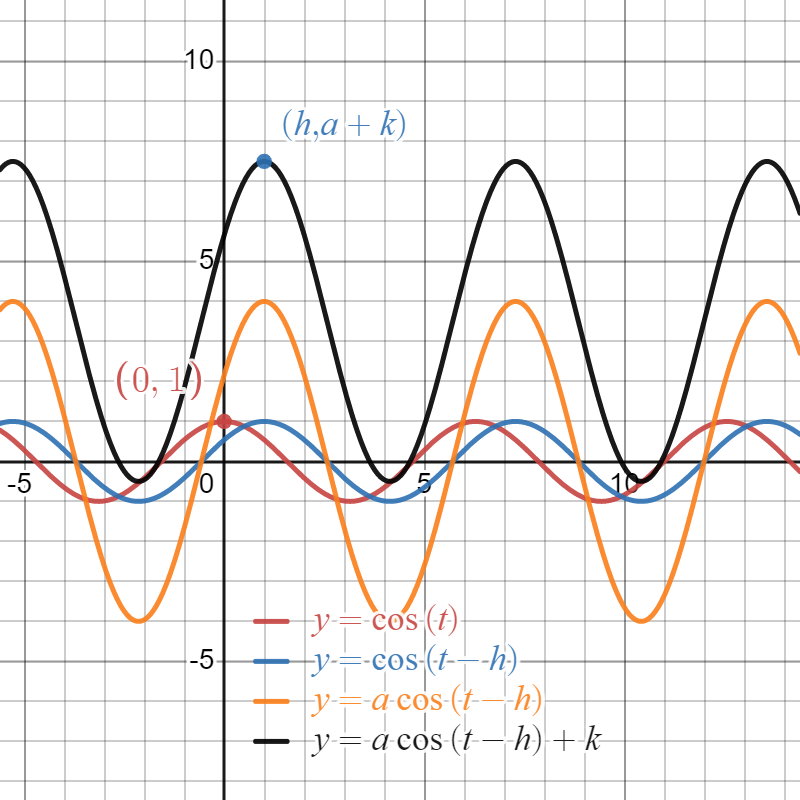
\includegraphics[width=0.8\linewidth]{images/sinusoidal-transformed-cosine-2.png}
\end{image}
It is often useful to follow one particular point through a sequence of transformations.  In the above figure, we see the red point that is located at \((0,1)\) on the original function \(y = \cos(t)\), as well as the point \((h, a+k)\) that is the corresponding point on \(f(t) = a\cos(t-h) + k\) under the overall transformation.  Note that the point \((h,a+k)\) results from the input, \(t = h\), that makes the argument of the cosine function zero:  \(f(h) = a\cos(h - h) + k = a\cos(0) + k = a + k\).%

While the sine and cosine functions extend infinitely in either direction, it's natural to think of the point \((0,1)\) as the ``starting point'' of the cosine function, and similarly the point \((0,0)\) as the starting point of the sine function.  We will refer to the corresponding points \((h,a+k)\) and \((h,k)\) on \(f(t) = a\cos(t-h) + k\) and \(g(t) = a\sin(t-h) + k\) as anchor points. Anchor points, along with other information about a circular function's amplitude, midline, and period help us to determine a formula for a function that fits a given situation.%

\begin{example}
Consider a spring-mass system where the weight resting on a frictionless table.  We let \(s(t)\) denote the distance from the wall (where the spring is attached) to the weight at time \(t\) in seconds and know that the weight oscillates periodically with a minimum value of \(s(t) = 2\) feet and a maximum value of \(s(t) = 7\) feet with a period of \(2 \pi\).  We also know that \(s(0) = 4.5\) and \(s\left(\frac{\pi}{2}\right) = 2\).%

Determine a formula for \(s(t)\) in the form \(s(t) = a\cos(t-b)+c\) or \(s(t) = a\sin(t-b)+c\).  Is it possible to find two different formulas that work?  

\begin{explanation}
Let's begin by drawing an accurate picture:
\begin{image}
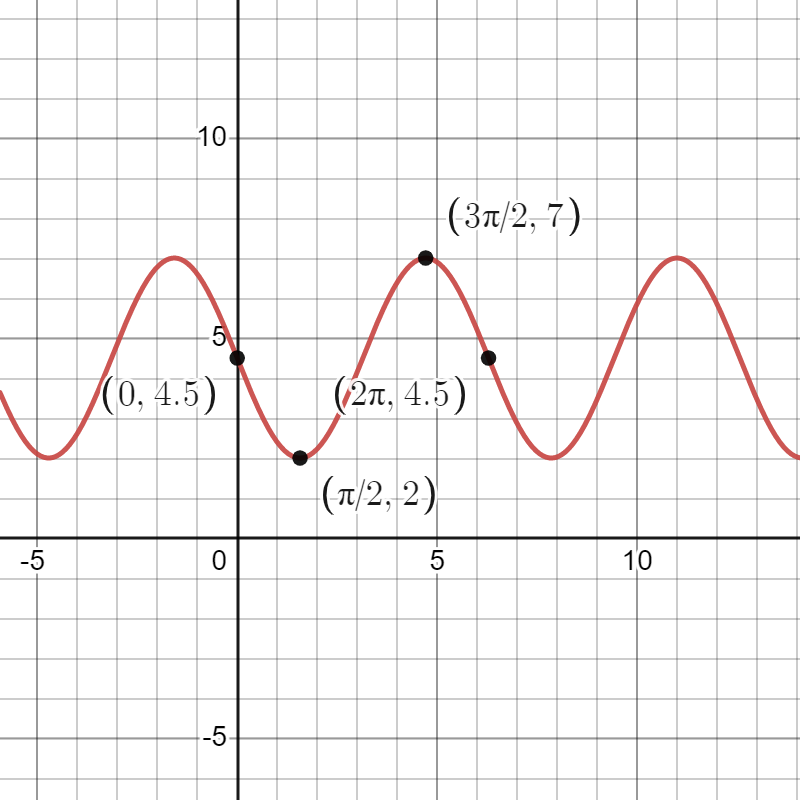
\includegraphics[width=0.8\linewidth]{images/spring-ex.png}
\end{image}

Since the minimum value of $s$ is 2 and the maximum value is 7, the midline of $s$ must be their midpoint, or $\frac{7+2}{2} = \frac{9}{2} = 4.5$. Now we can find the amplitude by finding the distance from the midline to the minimum (or maximum), which would be $|4.5 - 2| = 2.5$. 

Now we can try to find a formula that uses the sine function. Because the amplitude of $\sin(x)$ is 1, we must stretch by a factor of 2.5 to obtain the correct amplitude of $s$. This results in a transformed function of $s_1(x) = 2.5\sin(x)$. Because the midline of $\sin(x)$ is 0, we must shift up by 4.5 to get the midline that we want, resulting in the transformed function $s_2(x) = s_1(x) + 4.5 = 2.5\sin(x) + 4.5$. Now $s_2$ has the correct amplitude, midline, and period (unchanged from $2\pi$). The graph of $s_2$ looks like this:
\begin{image}
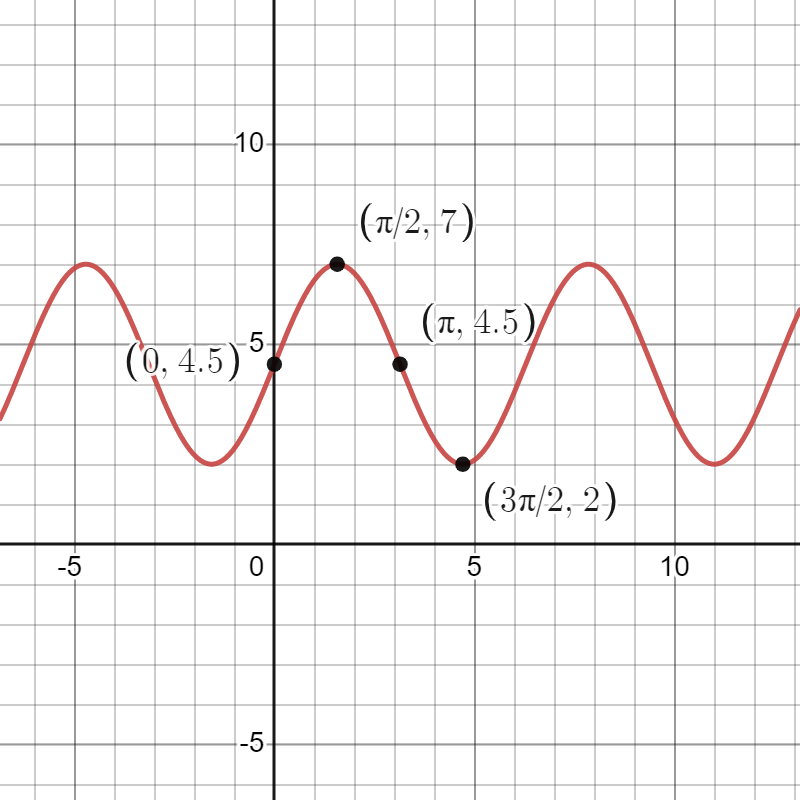
\includegraphics[width=0.8\linewidth]{images/spring-ex2.png}
\end{image}

After some examination, we can see that the only change we need to make to obtain the graph of $s$ is to shift $\pi$ units to the left, so that the points $(0, 4.5)$ and $\left(\frac{\pi}{2}, 2\right)$ are on the graph of $s$. Therefore, $s_3(x) = s_2(x + \pi) = 2.5\sin(x + \pi) + 4.5$ is a formula for $s$ in terms of the sine function. 

Note that we said that $2.5\sin(x + \pi) + 4.5$ was only \emph{a} formula for $s$. Let's try to find a formula using $\cos$. Since the amplitude of $\cos(x)$ is also 1, we still need to stretch by a factor of 2.5, yielding $s_1(x) = 2.5\cos(x)$. Again, since the midline of $s_1$ is 0, we need to shift up by 4.5 units, yielding $s_2(x) = s_1(x) + 4.5 = 2.5\cos(x) + 4.5$. The graph of $s_2$ this time looks as follows:
\begin{image}
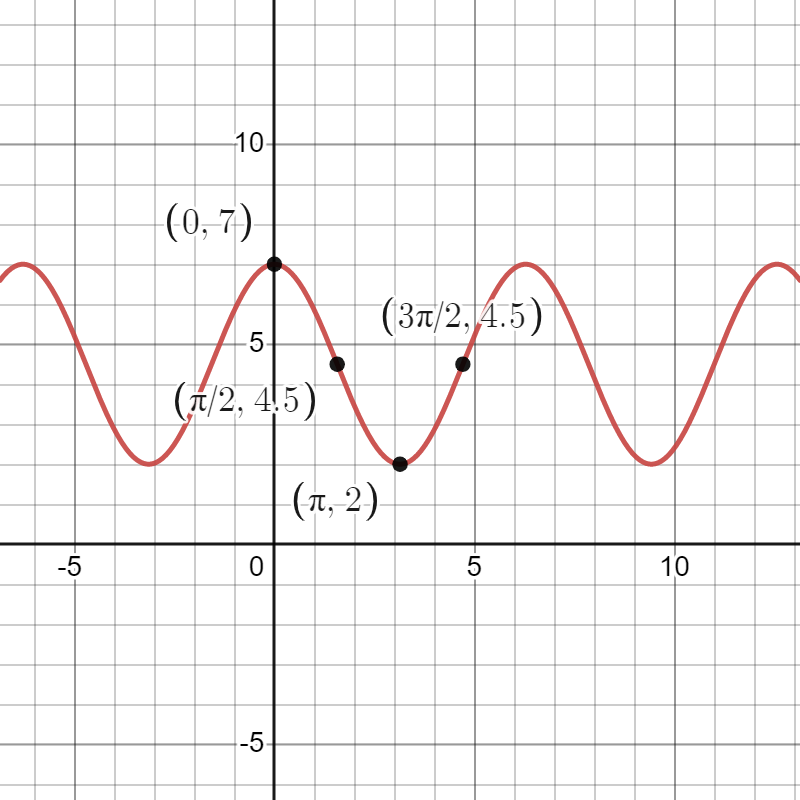
\includegraphics[width=0.8\linewidth]{images/spring-ex3.png}
\end{image}
After examining the picture, we see that to obtain the graph of $s$, we need to shift left by $\frac{\pi}{2}$ units, meaning that $s_3(x) = s_2\left(x + \frac{\pi}{2}\right) = 2.5\cos\left(x + \frac{\pi}{2}\right) + 4.5$ is another formula for $s$, this time in terms of the cosine function. 
\end{explanation}
\end{example}

The previous example illustrates a general technique for giving the formula of the graph of a circular function of period $2\pi$ with a given midline, amplitude, and $y$-intercept. Say $f$ is a circular function with period $2\pi$. If the midline is $m$, the amplitude is $a$, and we know that $f(0) = z$, then we have a procedure to follow to produce a formula for $f$. 
\begin{enumerate}
\item Stretch the graph vertically by a factor of $a$ to obtain $a\sin(x)$
\item Shift the graph vertically up by $m$ units to obtain $a\sin(x) + m$
\item Find $x$ such that $a\sin(x) + m = z$
\item Shift the function horizontally so that the point $(x, z)$ transforms into $(0, z)$. 
\end{enumerate}

Note that this procedure can work with $\cos$ as well as $\sin$. Let's see an example.

\begin{example}
Give the formula for a circular function $f$ with period $2\pi$ whose midline is $-2$, whose amplitude is 5, and whose $y$-intercept is $(0, -7)$.

\begin{explanation}
Since the amplitude is 5, the first transformation we apply to $\cos(x)$ is a vertical stretch by a factor of 5 to obtain $f_1(x) = 5\cos(x)$. Then, we need to shift down by 2 to obtain the correct midline: $f_2(x) = f_1(x) - 2 = 5\cos(x) - 2$. Finally, by looking at a graph, we can tell that $f_2(\pi) = 5\cos(\pi) - 2 = -5 - 2 = -7$, so we need to shift $\pi$ units to the left. Doing this gives us $f(x) = f_2(x + \pi) = 5\cos(x + \pi) - 2$. To check our work, we can graph the function and calculate its midline, amplitude, and $y$-intercept. 
\end{explanation}
\end{example} 

\begin{example}
Graph the function $f$ given by $f(x) = 7\cos(x + \pi) - 1$. Keep track of the points $(0, 1)$, $\left(\frac{\pi}{2}, 0\right)$, and $(\pi, -1)$ in each step. Give the midline, amplitude, and period of $f$. 

\begin{explanation}
We first graph the parent function, which is defined in this case by $f_0(x) = \cos(x)$. This graph has the points $(0, 1)$, $\left(\frac{\pi}{2}, 0\right)$, and $(\pi, -1)$, and is shown below.
\begin{image}
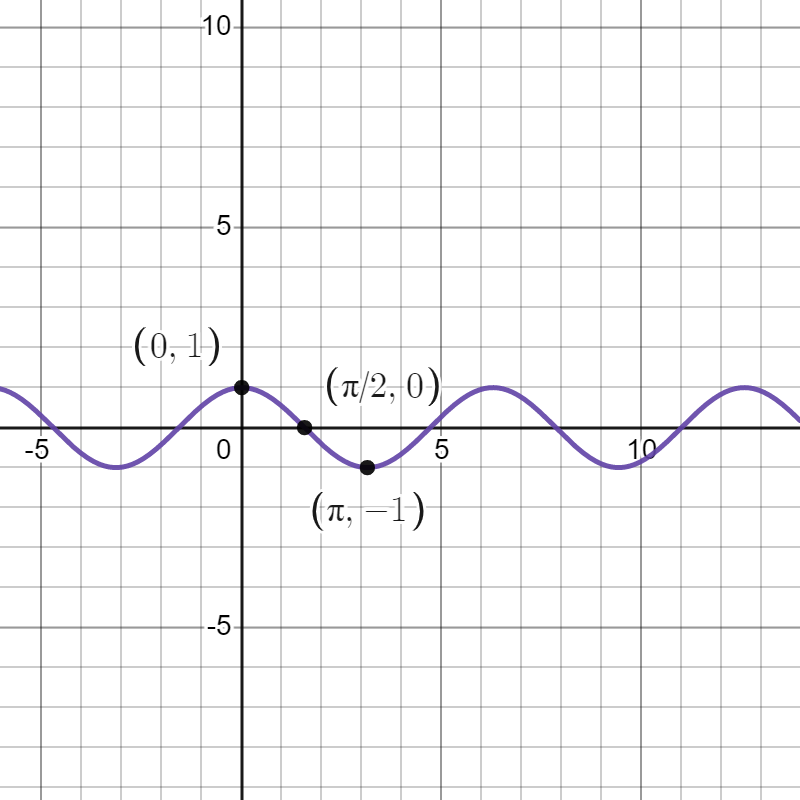
\includegraphics[width=0.8\linewidth]{images/graph-ex1.png}
\end{image}

We then proceed using the order of transformations outlined in a previous section. The first transformation to take place is the horizontal shift left by $\pi$ units. That results in the function $f_1(x) = f_0(x + \pi) = \cos(x + \pi)$ and moves our points to $(-\pi, 1)$, $\left(-\frac{\pi}{2}, 0\right)$, and $(0, -1)$.
\begin{image}
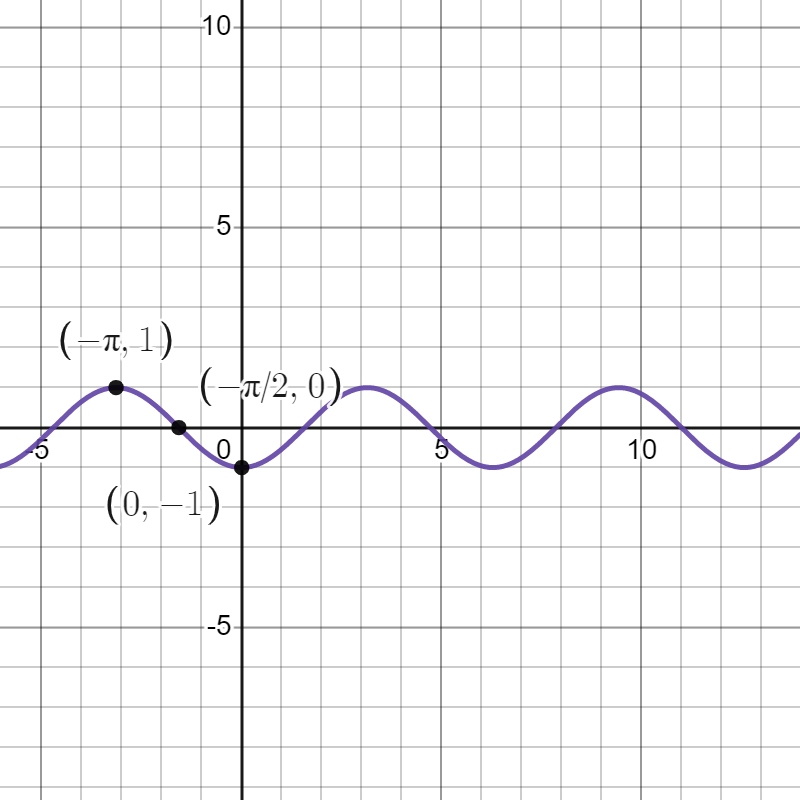
\includegraphics[width=0.8\linewidth]{images/graph-ex2.png}
\end{image} 

Next, we have a vertical stretch by a factor of 7. This results in the function $f_2(x) = 7f_1(x) = 7\cos(x + \pi)$ and moves our points to $(-\pi, 7)$, $\left(-\frac{\pi}{2}, 0\right)$, and $(0, -7)$.
\begin{image}
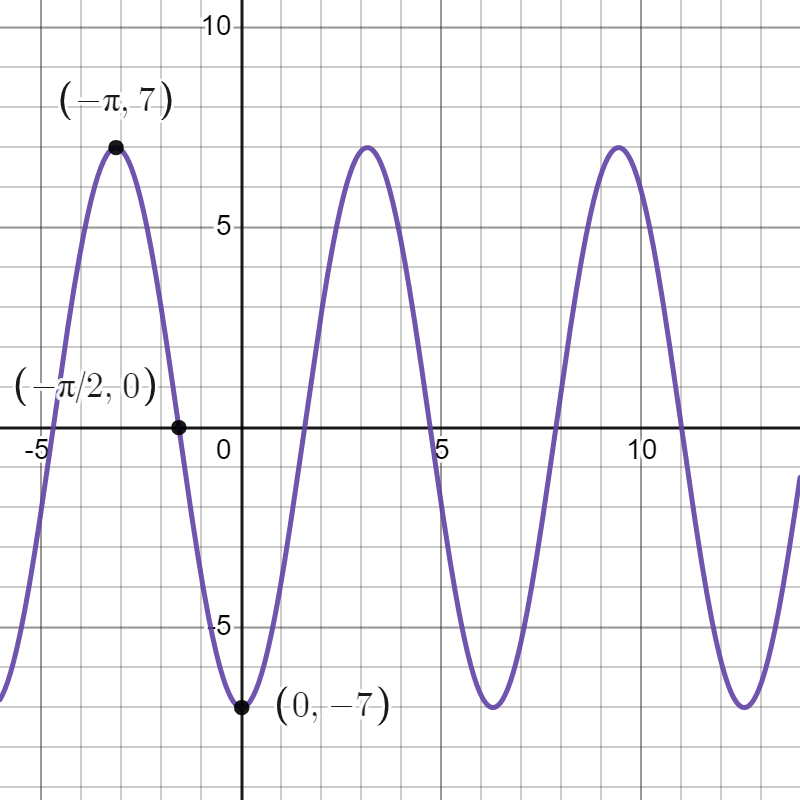
\includegraphics[width=0.8\linewidth]{images/graph-ex3.png}
\end{image} 

Finally, we shift down by 1 unit. This results in the function $f(x) = f_2(x) - 1 = 7\cos(x + \pi) - 1$ and moves our points to $(-\pi, 6)$, $\left(-\frac{\pi}{2}, -1\right)$, and $(0, -8)$.
\begin{image}
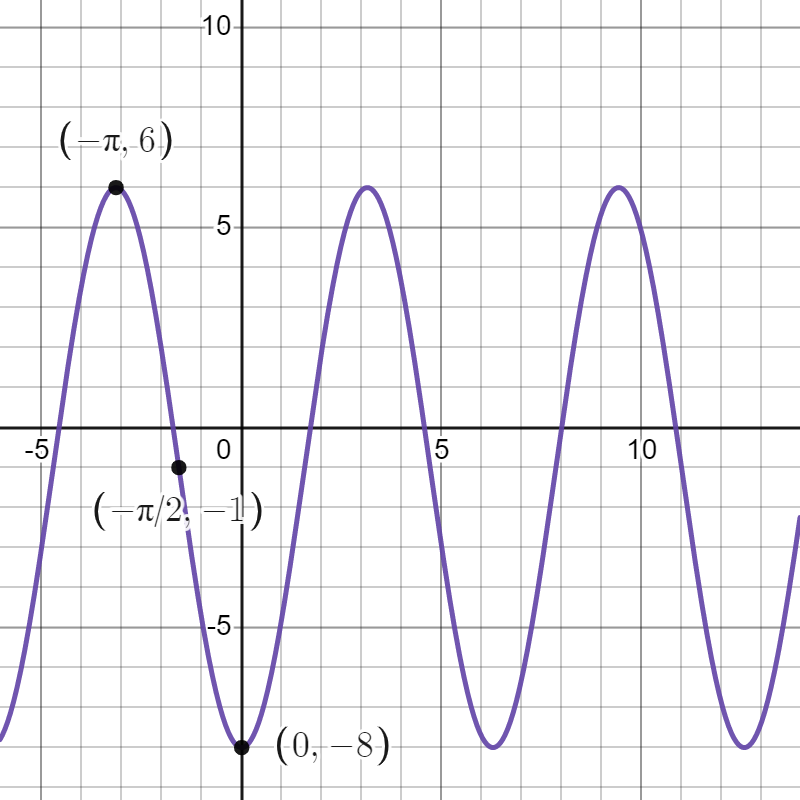
\includegraphics[width=0.8\linewidth]{images/graph-ex4.png}
\end{image} 
\end{explanation}

We can see from the graph that the midline of our function is $-1$, and the amplitude is 7. The period can also be read off as $2\pi$. Note that we could have read this information off from the formula, since $a = 7$, $k = -1$, and there is no horizontal stretch or compression.
\end{example}
%
%
%\typeout{************************************************}
%\typeout{Subsection 2.4.2 Horizontal scaling}
%\typeout{************************************************}
%

\section{Horizontal scaling}

There is one more very important transformation of a function that we've not yet explored in the trigonometric context.  Given a function \(y = f(x)\), we want to understand the related function \(g(x) = f(bx)\), where \(b\) is a positive real number.  The sine and cosine functions are ideal functions with which to explore these effects; moreover, this transformation is crucial for being able to use the sine and cosine functions to model phenomena that oscillate at different frequencies.%

By using a graphing utility such as Desmos, we can explore the effect of the transformation \(h(t) = f(bt)\), where \(f(t) = \sin(t)\).%

\begin{center}  
\desmos{zftuh2cfzr}{800}{600}  
\end{center}

By experimenting with the slider, we gain an intuitive sense for how the value of \(b\) affects the graph of \(h(t) = f(bt)\) in comparision to the graph of \(f(t)\).  When \(b = 2\), we see that the graph of \(h\) is oscillating twice as fast as the graph of \(f\) since \(h(t) = f(2t)\) completes two full cycles over an interval in which \(f\) completes one full cycle.  In contrast, when \(b = \frac{1}{2}\), the graph of \(h\) oscillates half as fast as the graph of \(f\), as \(h(t) = f\left(\frac{1}{2}t\right)\) completes only half of one cycle over an interval where \(f(t)\) completes a full one.%

We can also understand this from the perspective of function composition.  To evaluate \(h(t) = f(2t)\), at a given value of \(t\), we first multiply the input \(t\) by a factor of \(2\), and then evaluate the function \(f\) at the result.  An important observation is that%
\[
h\left( \frac{1}{2}t \right) = f\left( 2 \cdot \frac{1}{2}t \right) = f(t)\text{.}
\]
This tells us that the point \(\left(\frac{1}{2}t, f(t)\right)\) lies on the graph of \(h\) since an input of \(\frac{1}{2}t\) in \(h\) results in the value \(f(t)\).  At the same time, the point \((t,f(t))\) lies on the graph of \(f\).  Thus we see that the correlation between points on the graphs of \(f\) and \(h\) (where \(h(t) = f(2t)\)) is%
\[
(t, f(t)) \rightarrow \left( \frac{1}{2}t, f(t) \right)\text{.}
\]
We can therefore think of the transformation \(h(t) = f(2t)\) as achieving the output values of \(f\) twice as fast as the original function \(f(t)\) does.  Analogously, the transformation \(h(t) = f\left(\frac{1}{2}t\right)\) will achieve the output values of \(f\) only half as quickly as the original function.%

Recall that given a function \(y = f(t)\) and a real number \(b > 0\), the transformed function \(y = h(t) = f(bt)\) is a \emph{horizontal stretch} of the graph of \(f\).  Every point \((t,f(t))\) on the graph of \(f\) gets stretched horizontally to the corresponding point \(\left(\frac{1}{b}t,f(t)\right)\) on the graph of \(h\).  If \(0 < b < 1\), the graph of \(v\) is a stretch of \(f\) away from the \(y\)-axis by a factor of \(b\); if \(b > 1\), the graph of \(h\) is a compression of \(f\) toward the \(y\)-axis by a factor of \(b\).  The only point on the graph of \(f\) that is unchanged by the transformation is \((0,f(0))\).%


%While we will soon focus on horizontal stretches of the sine and cosine functions for the remainder of this section, it's important to note that horizontal scaling follows the same principles for any function we choose.%
%\begin{exploration}
%Consider the functions \(f\) and \(g\) given in the following figures.
%\begin{image}
%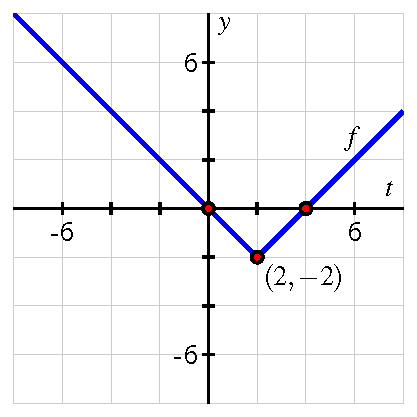
\includegraphics[width=1\linewidth]{images/sinusoidal-horiz-scaling-1.png}
%
%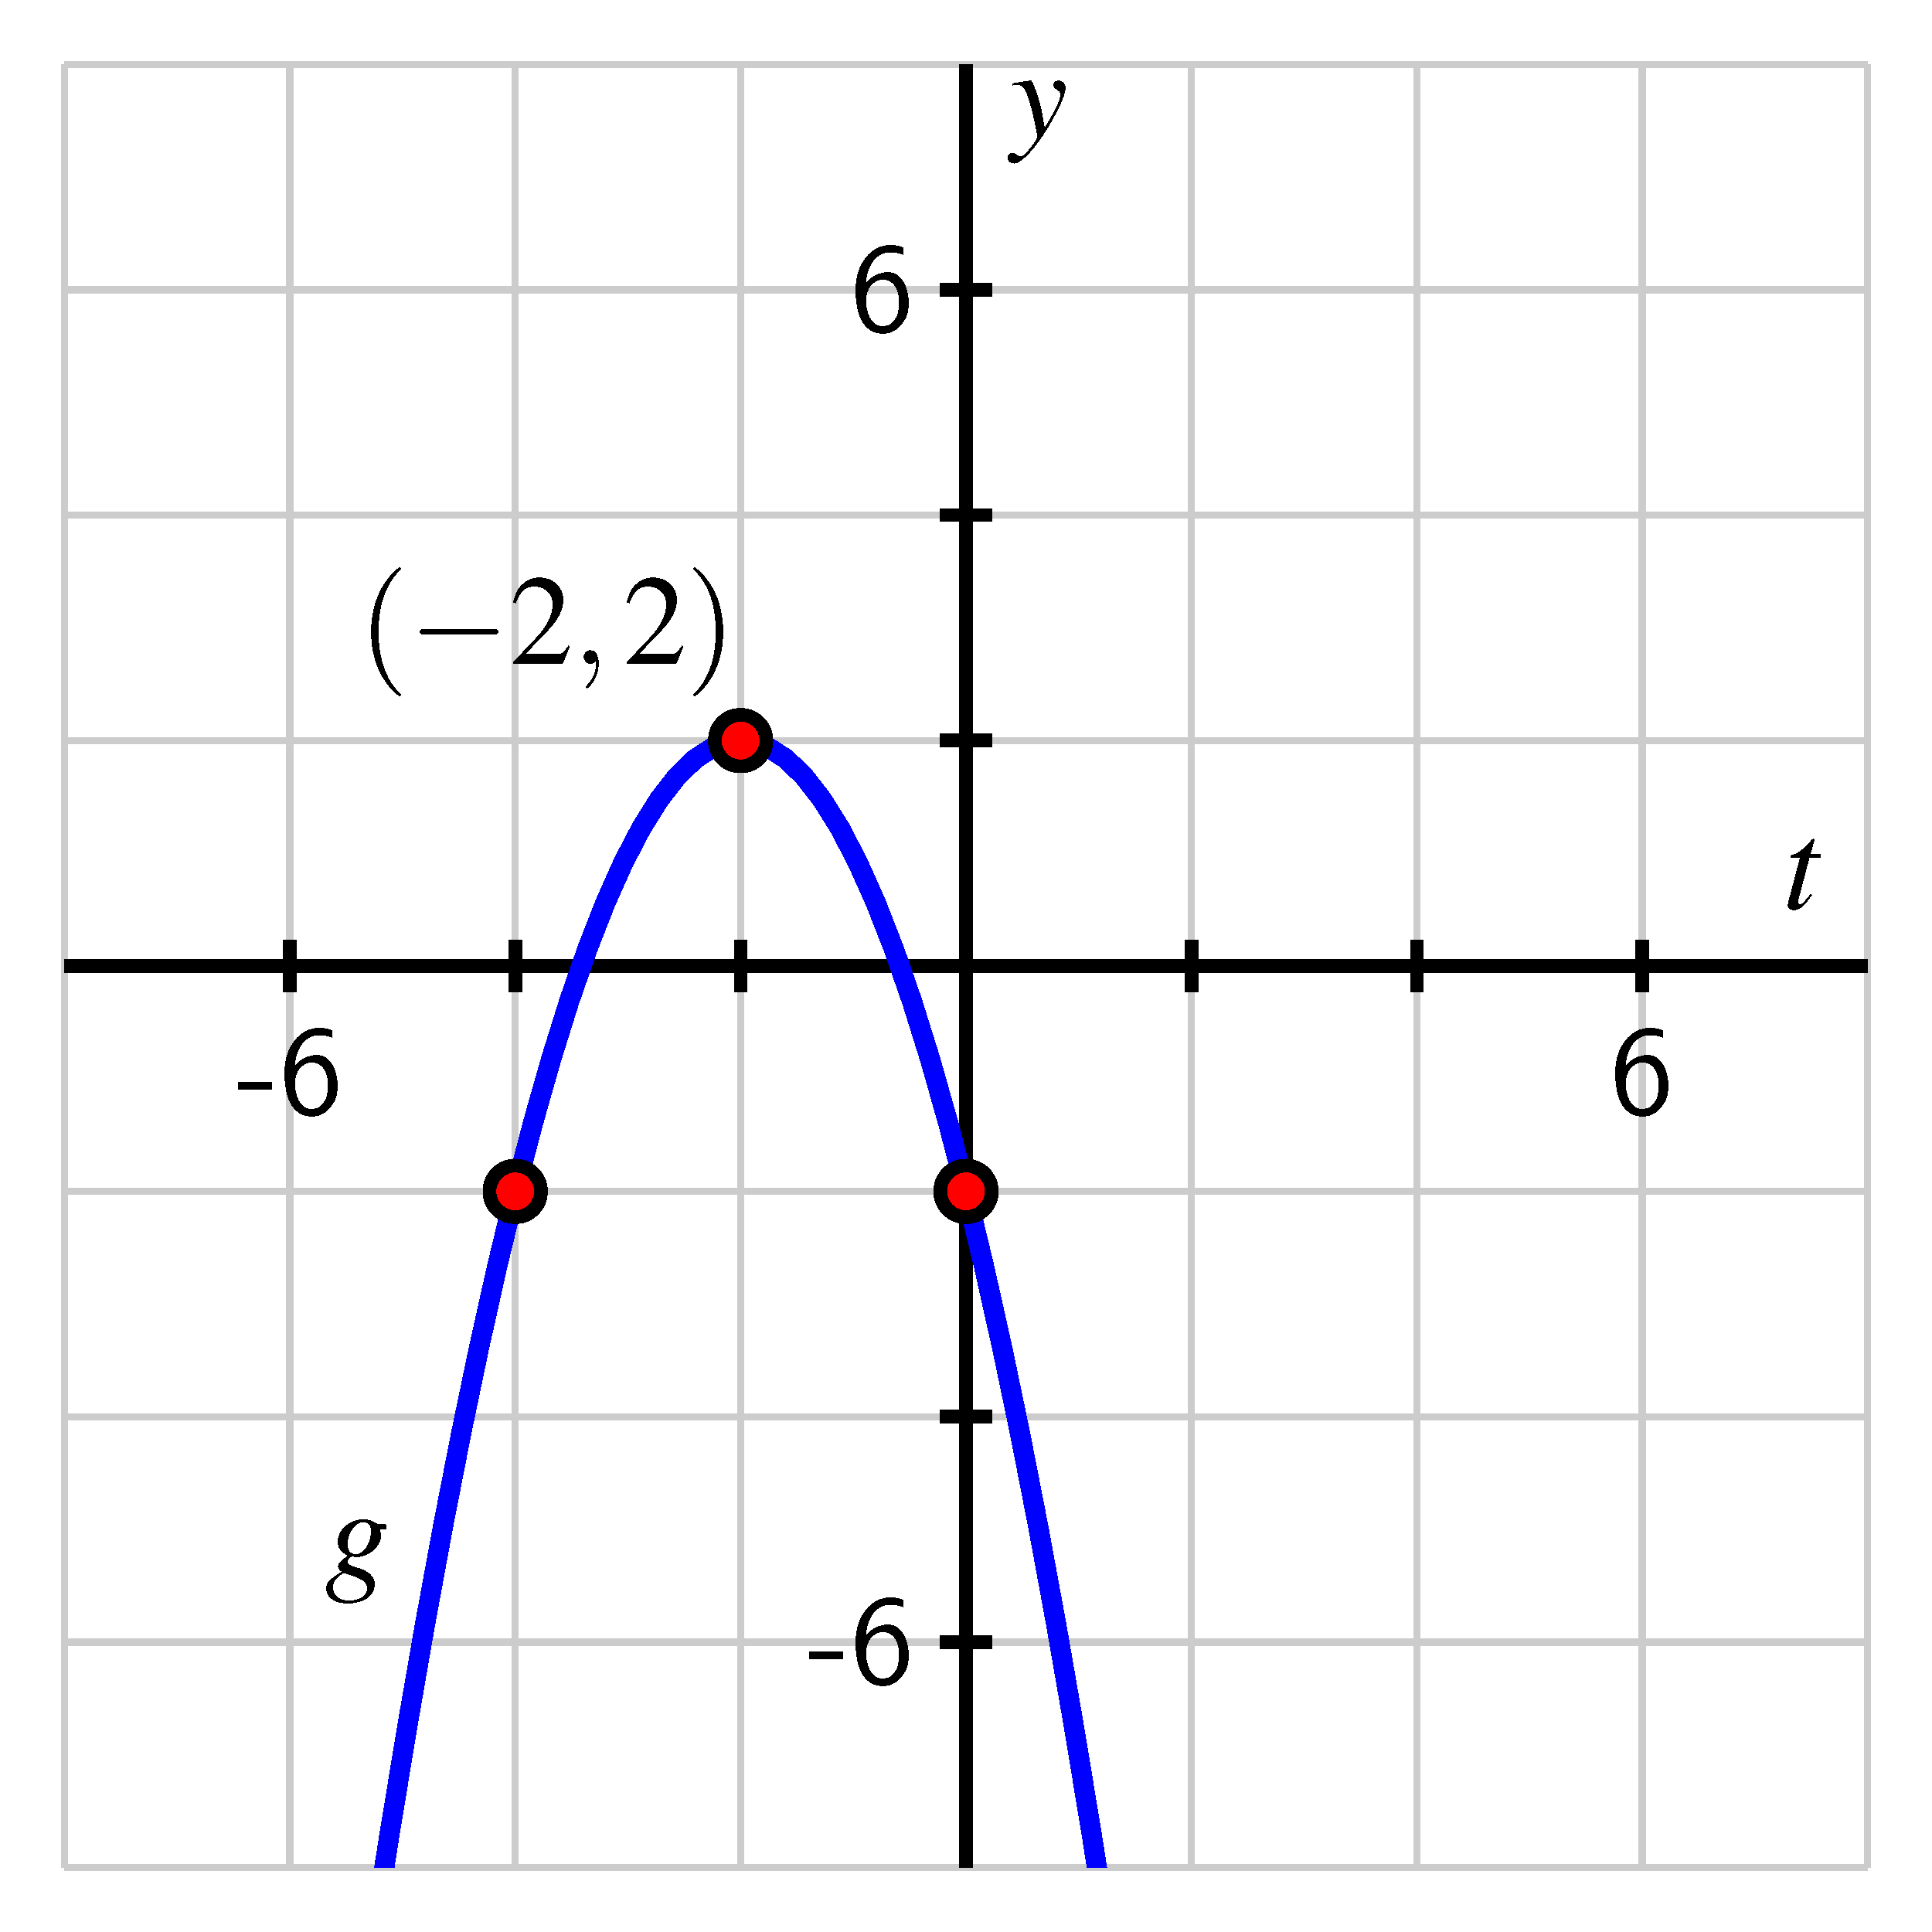
\includegraphics[width=1\linewidth]{images/sinusoidal-horiz-scaling-2.png}
%\end{image}
%\begin{enumerate}[label=\alph*.]
%\item
%On the same axes as the plot of \(y = f(t)\), sketch the following graphs:  \(y = h(t) = f(\frac{1}{3}t)\) and \(y = j(t) = r=f(4t)\).  Be sure to label several points on each of \(f\), \(h\), and \(k\) with arrows to indicate their correspondence.  In addition, write one sentence to explain the overall transformations that have resulted in \(h\) and \(j\) from \(f\).%
%\item
%On the same axes as the plot of \(y = g(t)\), sketch the following graphs:  \(y = k(t) = g(2t)\) and \(y = m(t) = g(\frac{1}{2}t)\).  Be sure to label several points on each of \(g\), \(k\), and \(m\) with arrows to indicate their correspondence.  In addition, write one sentence to explain the overall transformations that have resulted in \(k\) and \(m\) from \(g\).%
%\item
%On the additional copies of the two figures below, sketch the graphs of the following transformed functions:  \(y = r(t) = 2f(\frac{1}{2}t)\)  and \(y = s(t) = \frac{1}{2}g(2t)\).  As above, be sure to label several points on each graph and indicate their correspondence to points on the original parent function.%
%\begin{image}
%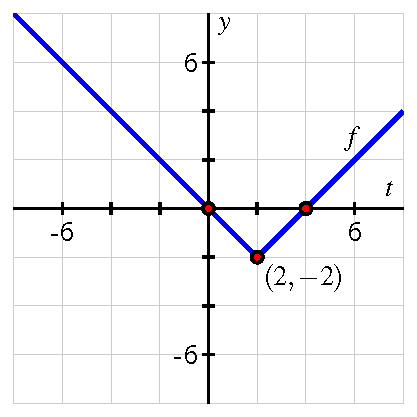
\includegraphics[width=1\linewidth]{images/sinusoidal-horiz-scaling-1.png}
%
%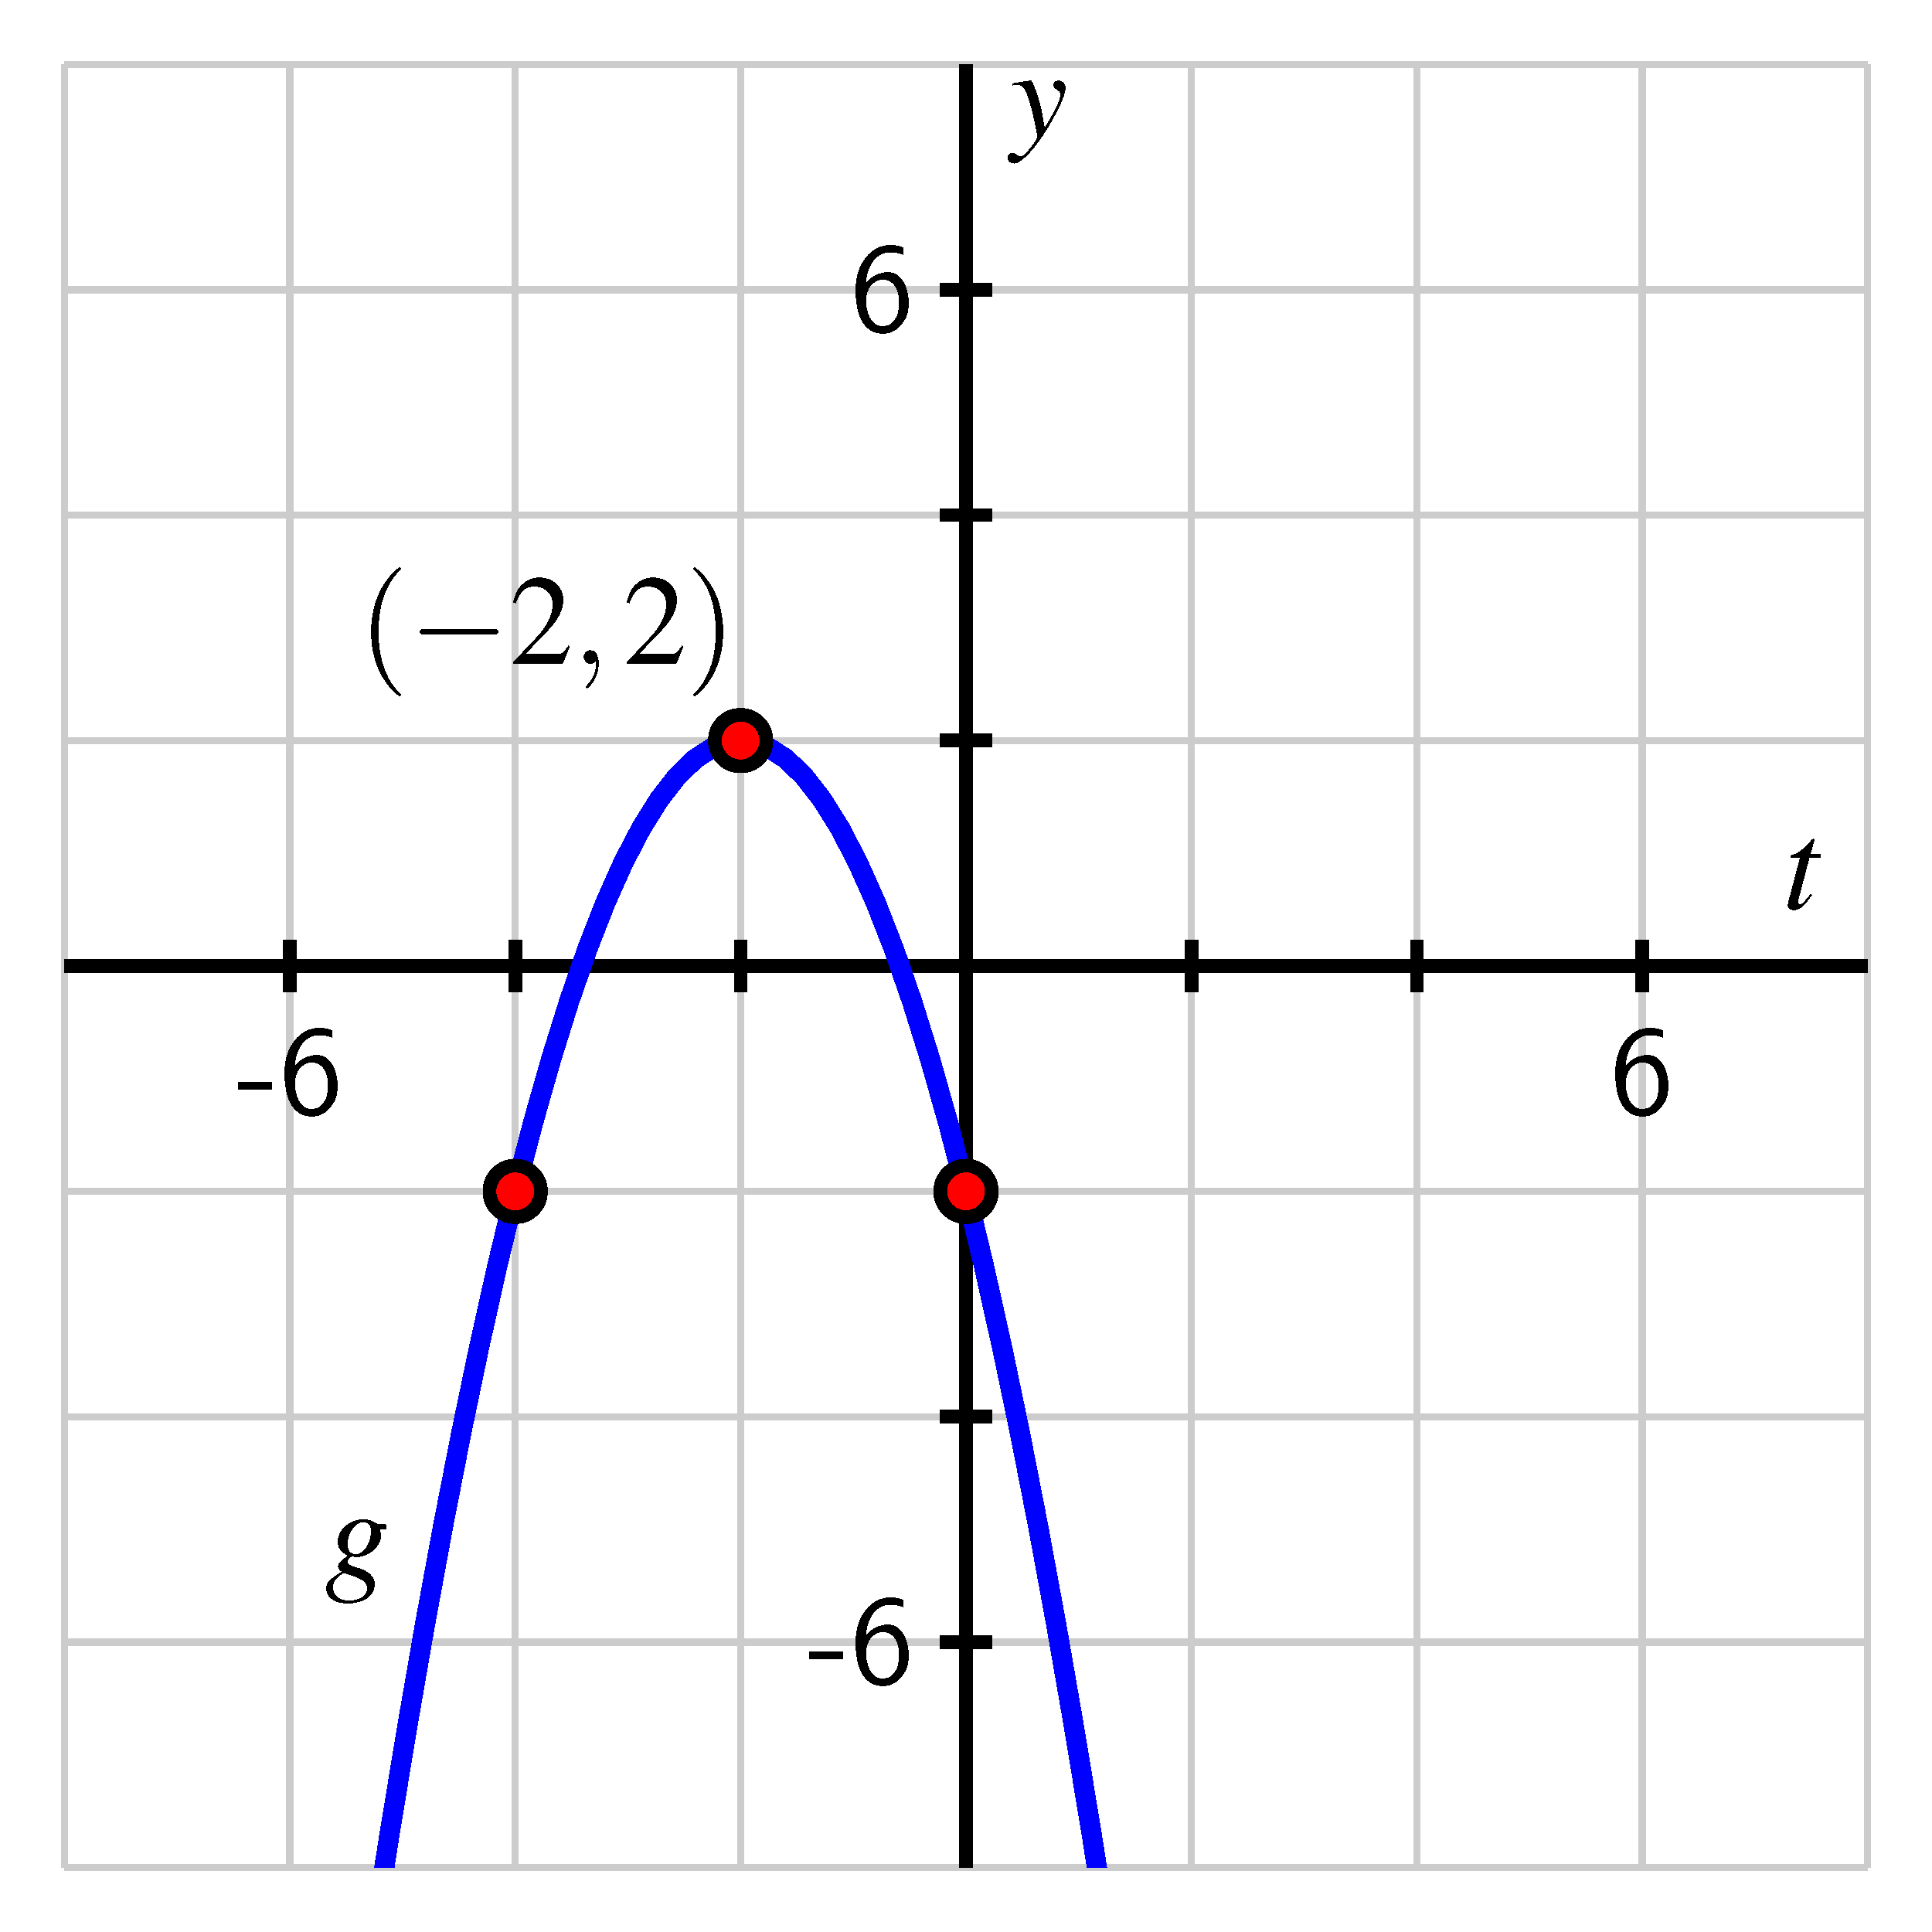
\includegraphics[width=1\linewidth]{images/sinusoidal-horiz-scaling-2.png}
%\end{image}
%\item
%Describe in words how the function \(y = r(t) = 2f(\frac{1}{2}t)\) is the result of two elementary transformations of \(y = f(t)\).  Does the order in which these transformations occur matter?  Why or why not?%
%\end{enumerate}
%\end{exploration}
%

%
%
%\typeout{************************************************}
%\typeout{Subsection 2.4.3 Circular functions with different periods}
%\typeout{************************************************}
%
\section{Circular functions with different periods}

Because the circumference of the unit circle is \(2\pi\), the sine and cosine functions each have period \(2\pi\).  Of course, as we think about using transformations of the sine and cosine functions to model different phenomena, it is apparent that we will need to generate functions with different periods than \(2\pi\).  For instance, if a ferris wheel makes one revolution every \(5\) minutes, we'd want the period of the function that models the height of one car as a function of time to be \(P = 5\).  Horizontal scaling of functions enables us to generate circular functions with any period we desire.%

We begin by considering two basic examples.  First, let \(f(t) = \sin(t)\) and \(g(t) = f(2t) = \sin(2t)\).  We know from our most recent work that this transformation results in a horizontal compression of the graph of \(\sin(t)\) by a factor of \(\frac{1}{2}\) toward the \(y\)-axis.  If we plot the two functions on the same axes, it becomes apparent how this transformation affects the period of \(f\).%
\begin{figure}
\centering
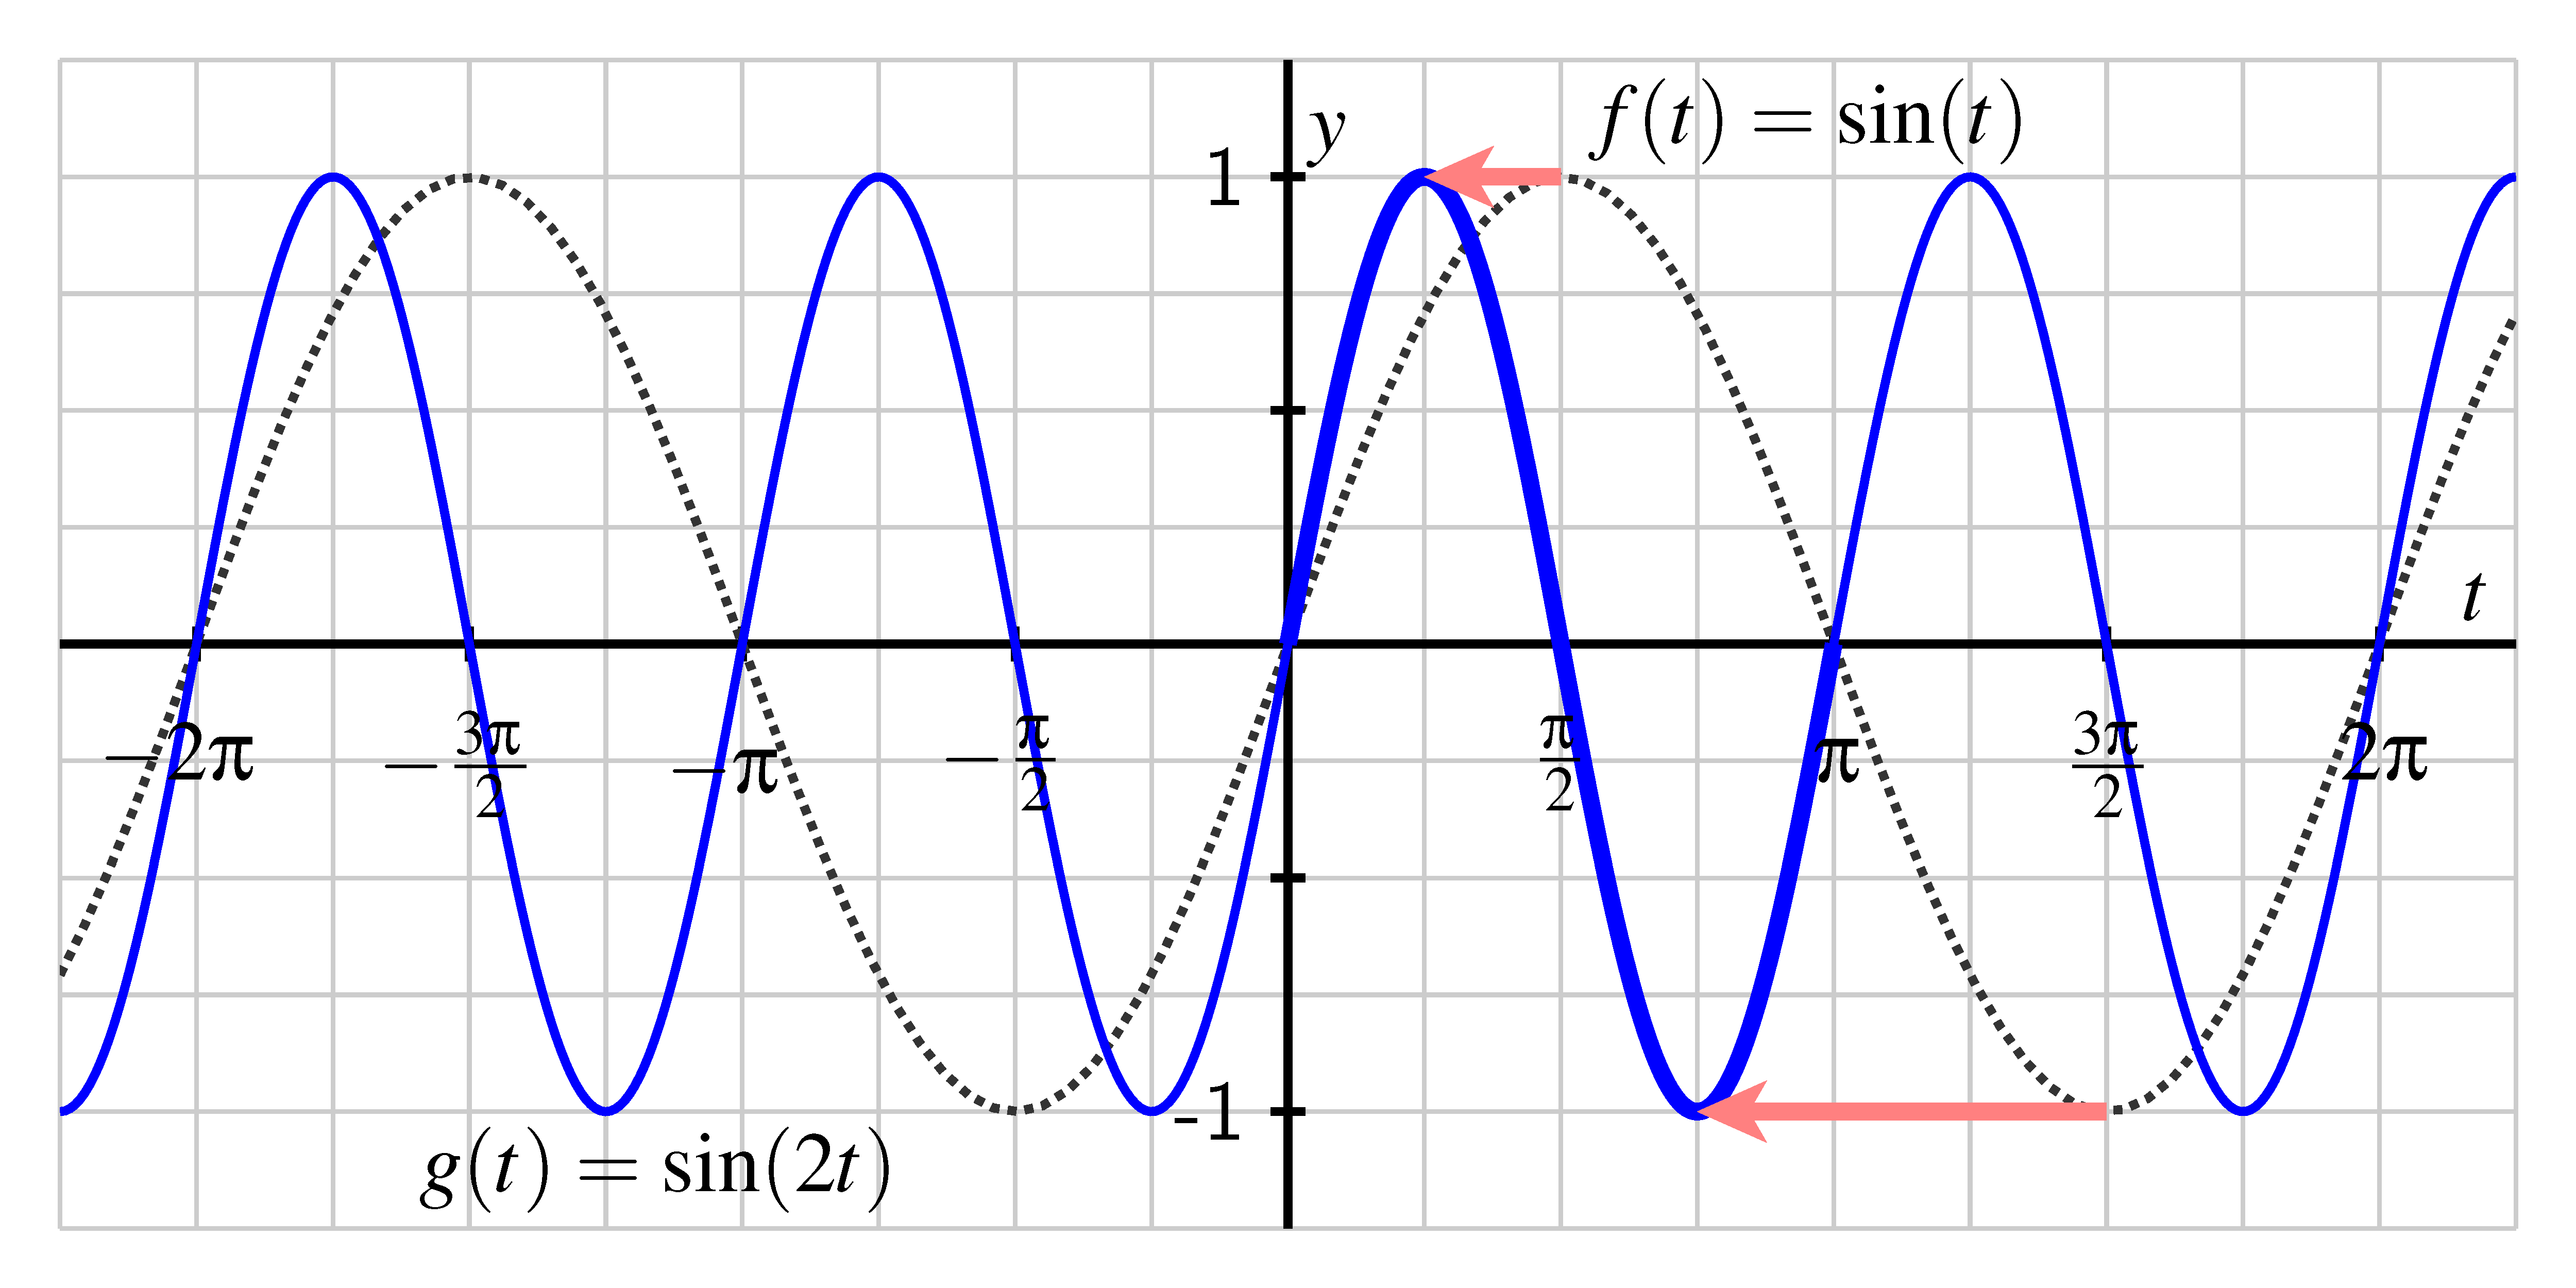
\includegraphics[width=0.75\linewidth]{images/sinusoidal-sine-horiz-scaling.png}
\caption{A plot of the parent function, \(f(t) = \sin(t)\) (dashed, in gray), and the transformed function \(g(t) = f(2t) = \sin(2t)\) (in blue).\label{F-sinusoidal-sine-compressed}}
\end{figure}

From the graph, we see that \(g(t) = \sin(2t)\) oscillates twice as frequently as \(f(t) = \sin(t)\), and that \(g\) completes a full cycle on the interval \([0,\pi]\), which is half the length of the period of \(f\).  Thus, the  ``\(2\)'' in \(f(2t)\) causes the period of \(f\) to be \(\frac{1}{2}\) as long; specifially, the period of \(g\) is \(P = \frac{1}{2} (2\pi) = \pi\).%
\begin{figure}
\centering
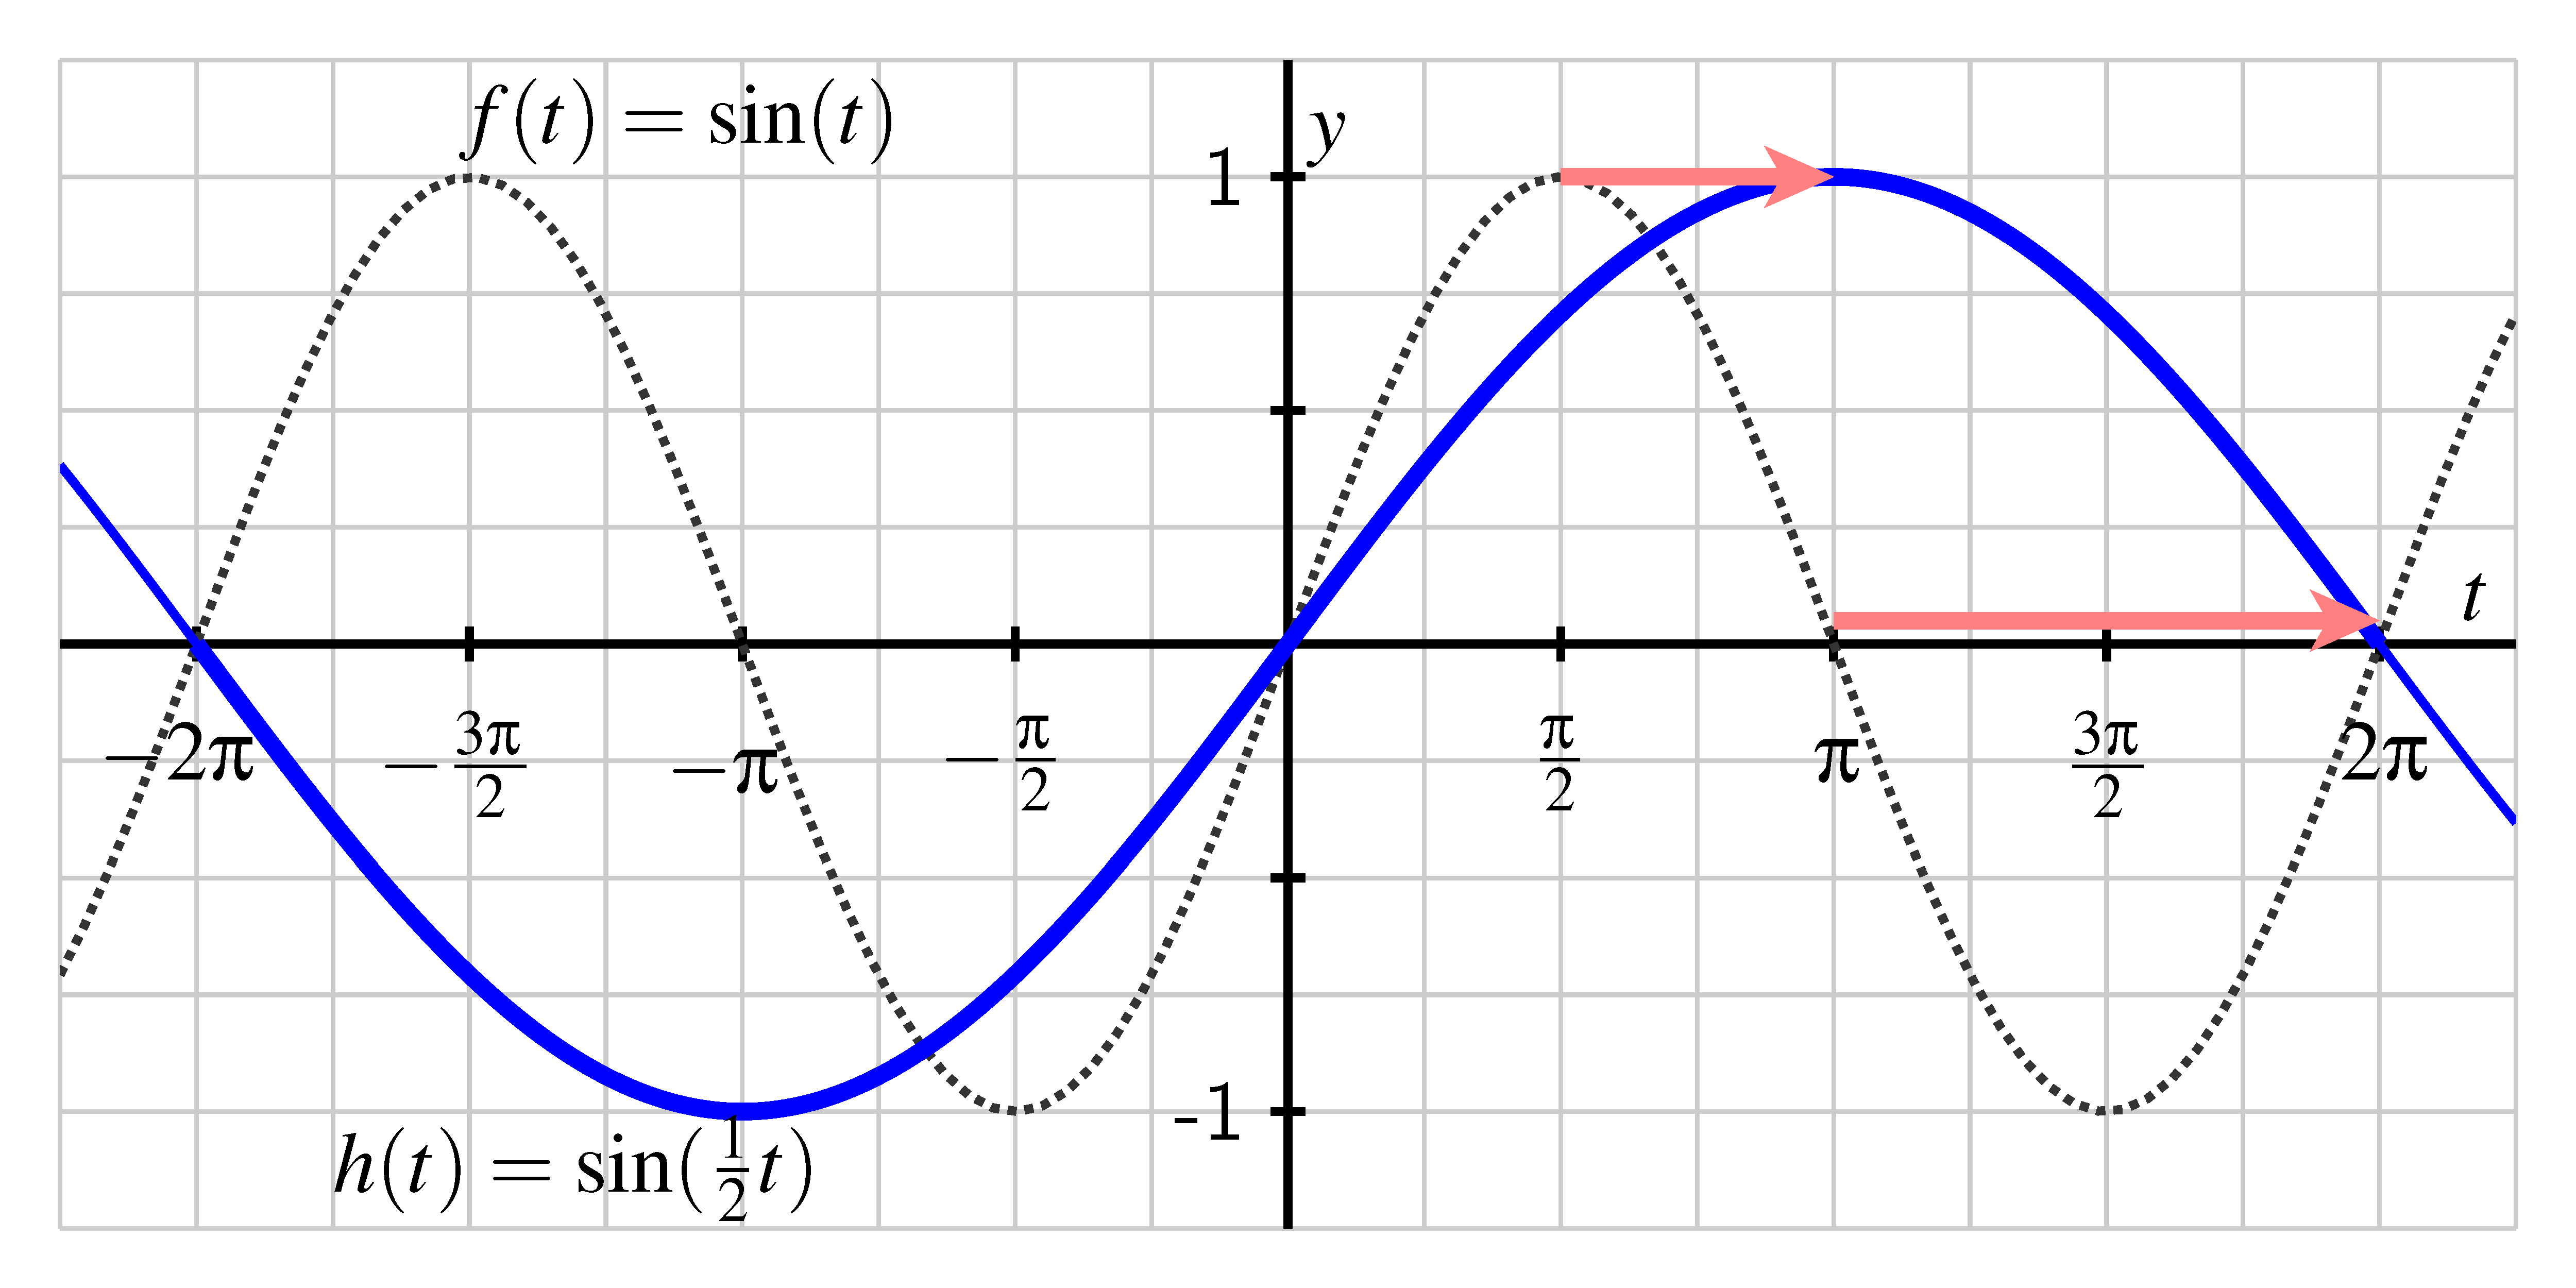
\includegraphics[width=0.75\linewidth]{images/sinusoidal-sine-horiz-scaling-2.png}
\caption{A plot of the parent function, \(f(t) = \sin(t)\) (dashed, in gray), and the transformed function \(h(t) = f\left(\frac{1}{2}t\right) = \sin\left(\frac{1}{2}t\right)\) (in blue).\label{F-sinusoidal-sine-stretched}}
\end{figure}

On the other hand, if we let \(h(t) = f\left(\frac{1}{2}t\right) = \sin\left(\frac{1}{2}t\right)\), the transformed graph \(h\) is stretched away from the \(y\)-axis by a factor of \(2\).  This has the effect of doubling the period of \(f\), so that the period of \(h\) is \(P = 2 \cdot 2\pi = 4\pi\), as seen in the previous figure.%

Our observations generalize for any positive constant \(b > 0\).  In the case where \(b = 2\), we saw that the period of \(g(t) = \sin(2t)\) is \(P = \frac{1}{2} \cdot 2\pi\), whereas in the case where \(b = \frac{1}{2}\), the period of \(h(t) = \sin(\frac{1}{2}t)\) is \(P = 2 \cdot 2\pi = \frac{1}{\frac{1}{2}} \cdot 2\pi\).  Identical reasoning holds if we are instead working with the cosine function.  In general, we can say the following.%

For any constant \(b > 0\), the period of the functions \(\sin(bt)\) and \(\cos(bt)\) is%
\[
P = \frac{2\pi}{b}\text{.}
\]
%

Thus, if we know the \(b\)-value from the given function, we can deduce the period.  If instead we know the desired period, we can determine \(b\) by the rule \(b = \frac{2\pi}{P}\).%

\begin{callout}
\textbf{Transformations of sine and cosine with any shift or stretch.}\\
Given real numbers \(a\), \(b\), \(h\), and \(k\) with \(a > 0\) and \(b > 0\) , the functions%
\begin{equation*}
f(t) = a\cos(b(t-h))+k \text{ or } g(t) = a\sin(b(t-h)) + k\text{.}
\end{equation*}
each represent a horizontal stretch or compression by a factor of $b$, followed by a vertical stretch by \(a\) units, followed by a vertical shift of \(k\) units, applied to the parent function (\(\cos(t)\) or \(\sin(t)\), respectively). They then contain a horizontal shift to the right by $h$ units. The resulting circular functions have midline \(y = k\), amplitude \(a\), range \([k-a,k+a]\), and period \(P = 2\pi/b\). In addition, the point \((h,a+k)\) lies on the graph of \(f\) and the point \((h, k)\) lies on the graph of \(g\).
\end{callout}

\begin{callout}
Be careful! These calculations only apply to $\sin$ and $\cos$. For example, $\tan(bx)$ has a period of $\frac{\pi}{b}$, not $\frac{2\pi}{b}$, since the original period of $\tan$ is just $\pi$. When you're faced with a problem involving a transformation of a trig function, it's best to start from what you already know about the trig function, then see how each transformation affects its properties. 
\end{callout}

\begin{example}
Determine the exact period, amplitude, and midline of each of the following functions.  In addition,  state the range of each function and any horizontal shift that has been introduced to the graph.  Make your conclusions without consulting \emph{Desmos}, and then use the program to check your work.%

\begin{enumerate}[label=\alph*.]
\item
\(p(x) = \sin(10x) + 2\)%
\item
\(q(x) = -3\cos(0.25x) - 4\)%
\item
\(r(x) = 2\sin\left( \frac{\pi}{4} x\right) + 5\)%
\item
\(w(x) = 2\cos\left( \frac{\pi}{2} (x-3) \right) + 5\)%
\item
\(u(x) = -0.25\sin\left(3x-6\right) + 5\)%
\end{enumerate}
\begin{explanation}
\begin{enumerate}[label=\alph*.]
\item
$p(x)$ has a period of $\frac{\pi}{5}$, an amplitude of $1$ and a midline of $y=2$. \\
The range of $p(x)$ is $[1,3]$.
\item
$q(x)$ has a period of $8\pi$, an amplitude of $3$ and a midline of $y=-4$. \\
The range of $q(x)$ is $[-7, -1]$.
\item
$r(x)$ has a period of $8$, an amplitude of $2$ and a midline of $y=5$. \\
 The range of $r(x)$ is $[3, 7]$.
\item
$w(x)$ has a period of $4$, an amplitude of $2$ and a midline of $y=5$.\\
The range of $w(x)$ is $[3, 7]$. \\
There is a horizontal shift of $3$ to the right.
\item
$u(x)$ has a period of $\frac{2\pi}{3}$, an amplitude of $0.25$ and a midline of $y=5$. \\
The range of $u(x)$ is $[4.75, 5.25]$. \\
There is a horizontal shift of $2$ to the right. This is because we have to factor out the 3 inside the parentheses: $-0.25\sin(3(x - 2)) + 5$. 
\end{enumerate}
\end{explanation}
\end{example}

You might wonder why we've chosen to use the formula $a\sin(b(t-h)) + k$ with the parentheses instead of $a\sin(bt - h) + k$ without the parentheses. In the former formula, we save the horizontal shift until the end, but in the latter, we do the horizontal shift before anything else. The reason we prefer the former is that the midline, amplitude, and period of a function are easy to plug into the formula, and plugging these in results in a formula of the form $f_1(t) = a\sin(bt) + k$. We can then find the horizontal shift we need to apply to the graph of $f_1$ to obtain $f(t) = f_1(t - h) = a\sin(b(t - h)) + k$. 

\begin{example}
Consider a spring-mass system where the weight is hanging from the ceiling in such a way that the following is known: we let \(d(t)\) denote the distance from the ceiling to the weight at time \(t\) in seconds and know that the weight oscillates periodically with a minimum value of \(d(t) = 1.5\) and a maximum value of \(d(t) = 4\), with a period of \(3\), and you know \(d(0.5) = 2.75\) and \(d\left(1.25\right) = 4\).%

State the midline, amplitude, range, and an anchor point for the function, and hence determine a formula for \(d(t)\) in the form \(a\cos(b(t-h))+k\) or \(a\sin(b(t-h))+k\). Show your work and thinking, and use \emph{Desmos} appropriately to check that your formula generates the desired behavior.%

\begin{explanation}
Since the period of our function is 3, we know that $b = \frac{2\pi}{3}$. The midline is the midpoint of the minimum and maximum values: $\frac{4 + 1.5}{2} = \frac{5.5}{2} = 2.75$. The amplitude is the distance from the midline to the maximum (or minimum): $|2.75 - 4| = 1.25$. Plugging all this information into a function, we obtain $d_1(t) = 1.25\cos\left(\frac{2\pi}{3}t\right) + 2.75$. 

Since we started with the cosine function, we know that the maximum of $1.25\cos\left(\frac{2\pi}{3}t\right) + 2.75$ is 4, and occurs at $t = 0$. Since we want $d(1.25) = 4$, we need to shift our graph to the right by 1.25 units. This means $d(t) = d_1(t - 1.25) = 1.25\cos\left(\frac{2\pi}{3}(t - 1.25)\right) + 2.75$. We can then check that $d(0.5) = 2.75$ by plugging into our function. 
\end{explanation}
\end{example}

\begin{example}
Let $f$ be a circular function with midline $\pi$, amplitude $\frac{\pi}{2}$, and period 5, with $f(8) = \frac{3\pi}{2}$. Give a formula for $f$ of the form $a\cos(b(t - h)) + k$ or $a\sin(b(t - h)) + k$.

\begin{explanation}
Since $a$ corresponds to the amplitude, $a = \frac{\pi}{2}$. Since $k$ corresponds to the midline, $k = \pi$. Since the period is given by $\frac{2\pi}{b}$, $b = \frac{2\pi}{5}$. 

Let's now pay some attention to the choice between sine and cosine. Note that since the midline is $\pi$ and the amplitude is $\frac{\pi}{2}$, the maximum of our function is $\frac{3\pi}{2}$. This means that the condition that $f(8) = \frac{3\pi}{2}$ tells us where the maximum should be. We have a very easy location for the maximum of cosine: $t = 0$, so we'll choose to use cosine here. Note that choosing sine isn't incorrect, just more difficult.

Plugging our values into the equation, we have $f_1(t) = \frac{\pi}{2}\cos\left(\frac{2\pi}{5}t\right) + \pi$. The maximum for cosine occurs at $t = 0$, as stated above, but we want the maximum to occur at $t = 8$, so we'll shift the graph of $f_1$ 8 units to the right. This gives us $f(t) = f_1(t - 8) =  \frac{\pi}{2}\cos\left(\frac{2\pi}{5}(t - 8)\right) + \pi$.
\end{explanation}
\end{example}

\begin{example}
Give a formula of the form $a\cos(b(t - h)) + k$ or $a\sin(b(t - h)) + k$ for the graph below.

\begin{image}
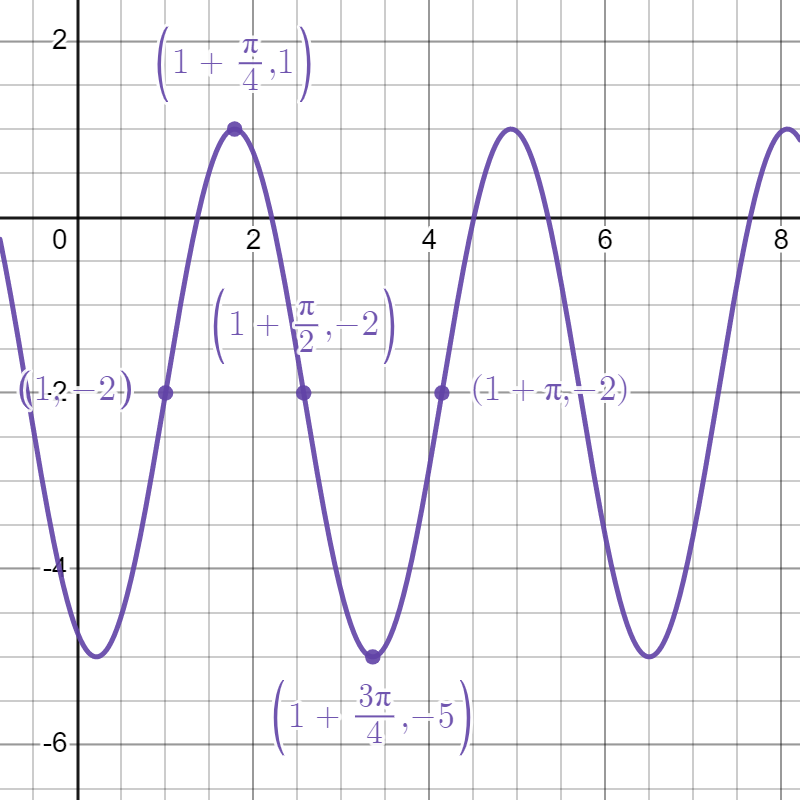
\includegraphics[width=0.8\linewidth]{images/graph-to-formula.png}
\end{image}

\begin{explanation}
Although this problem may seem different from the previous problem, we can still collect information about the midline, amplitude, and period from the graph of the function. 

Here, the amplitude is 3, the midline is $-2$, and the period is $\pi$. Using the sine function as a parent function, this gives us $f_1(t) = 3\sin(2t) - 2$. Note that $f_1(0) = 3\sin(0) - 2 = 0 - 2 = -2$, and we want our function to have $f(1) = -2$, so we need to shift the graph of $f_1$ to the right by 1 unit. This gives us $f(t) = f_1(t - 1) = 3\sin(2(t - 1)) - 2$. 
\end{explanation}
\end{example}

\begin{example}
Graph the function $f$ given by $f(x) = -2\sin(2(x - 1)) + 3$. Keep track of the points $(0, 0)$, $\left(\frac{\pi}{2}, 1\right)$, and $(\pi, 0)$ at each step. Give the midline, amplitude, and period of $f$. 

\begin{explanation}
While this may seem like a complicated set of transformations, it's nothing that we couldn't have done in the earlier section on function transformations. The only catch here is that in order to use our order from before, we need to distribute the 2 inside the parentheses to obtain $f(x) = -2\sin(2x - 2) + 3$. This puts our function in the form needed to use the order. 

With this change, we can see that our first transformation is a shift right by 2 units, yielding $f_1(x) = \sin(x - 2)$. This transforms our points into $(2, 0)$, $\left(\frac{\pi}{2} + 2, 1 \right)$, and $(\pi + 2, 0)$.  We can see a graph of $f_1$ below.
\begin{image}
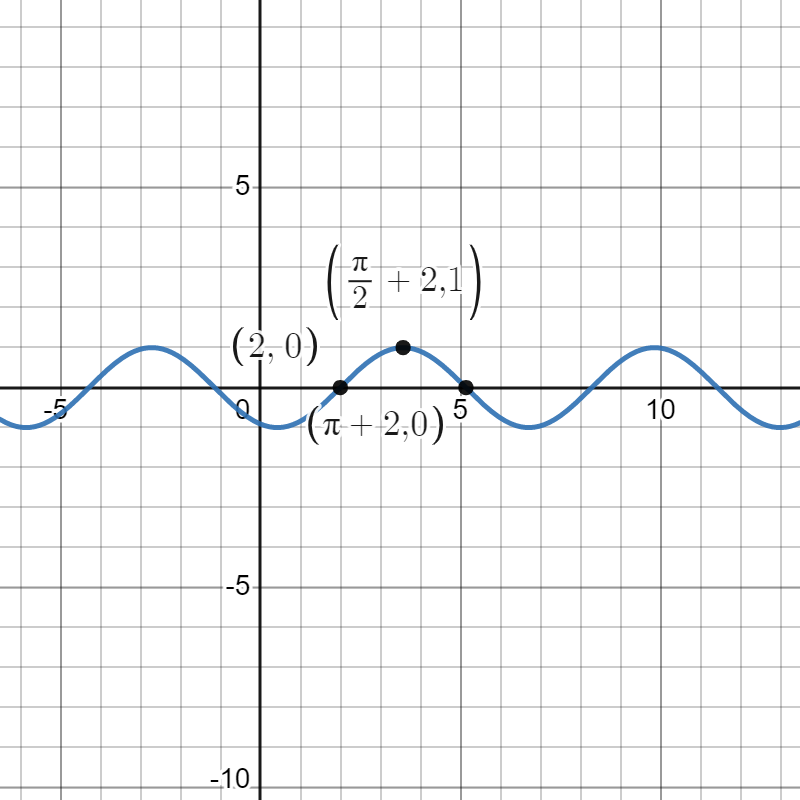
\includegraphics[width=0.8\linewidth]{images/graph-2-ex1.png}
\end{image}

Our next transformation in the order is a horizontal compression by a factor of 2, yielding $f_2(x) = f_1(2x) = \sin(2x - 2)$. This transforms our points into $(2, 0)$, $\left(\frac{\pi}{4} + 1, 1 \right)$, and $\left(\frac{\pi}{2} + 1, 0\right)$.  We can see a graph of $f_2$ below.
\begin{image}
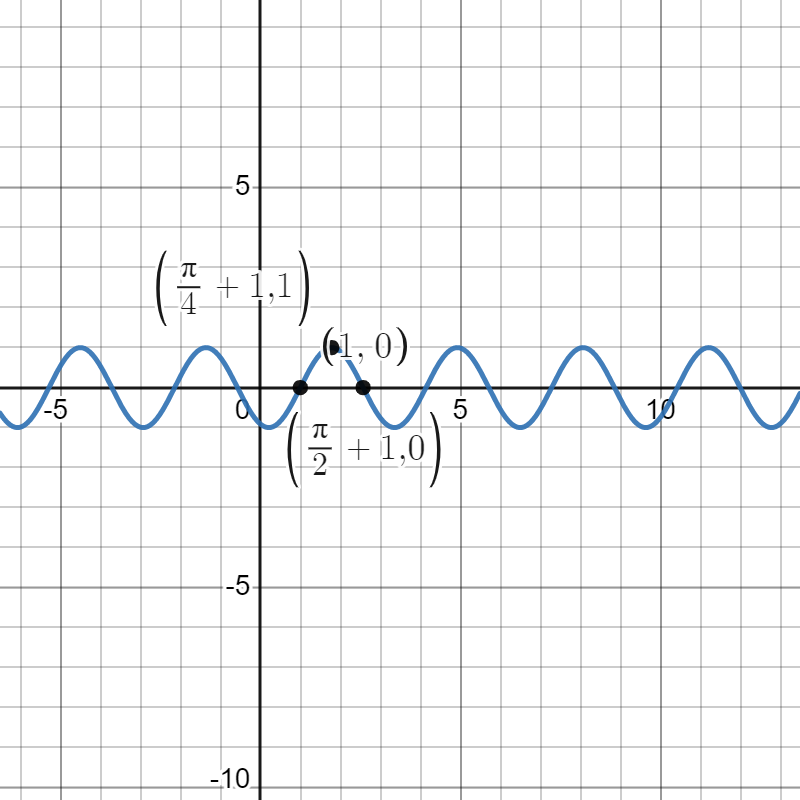
\includegraphics[width=0.8\linewidth]{images/graph-2-ex2.png}
\end{image}

Our next transformation is a vertical stretch by a factor of 2, yielding $f_3(x) = 2f_2(x) = 2\sin(2x - 2)$. This transforms our points into $(2, 0)$, $\left(\frac{\pi}{4} + 1, 2 \right)$, and $\left(\frac{\pi}{2} + 1, 0\right)$.  We can see a graph of $f_3$ below.
\begin{image}
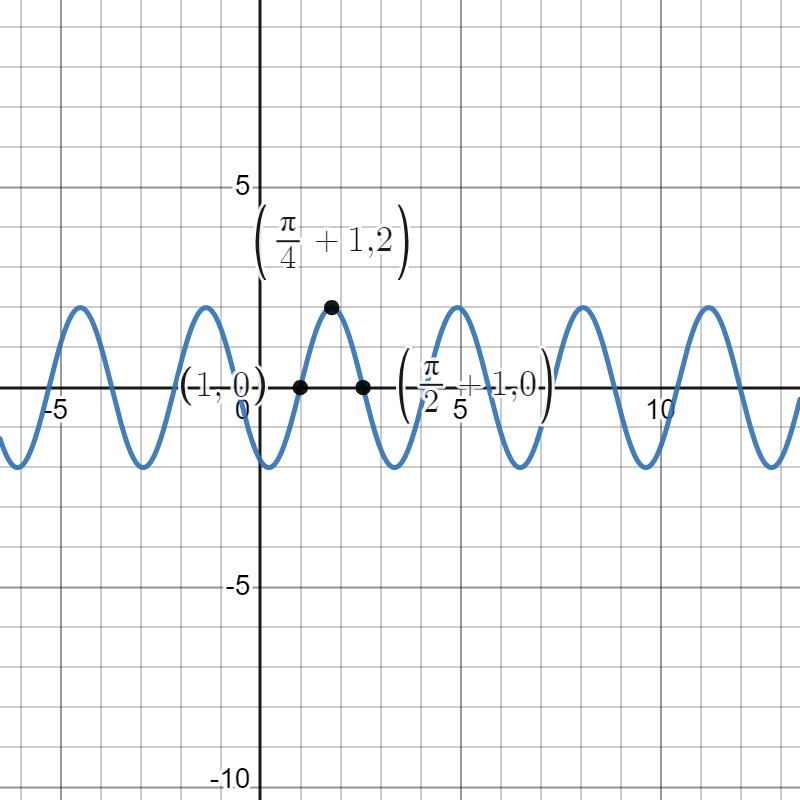
\includegraphics[width=0.8\linewidth]{images/graph-2-ex3.png}
\end{image}

Our next transformation is a reflection across the $x$-axis, yielding $f_4(x) = -f_3(x) = -2\sin(2x - 2)$. This transforms our points into $(2, 0)$, $\left(\frac{\pi}{4} + 1, -2 \right)$, and $\left(\frac{\pi}{2} + 1, 0\right)$.  We can see a graph of $f_4$ below.
\begin{image}
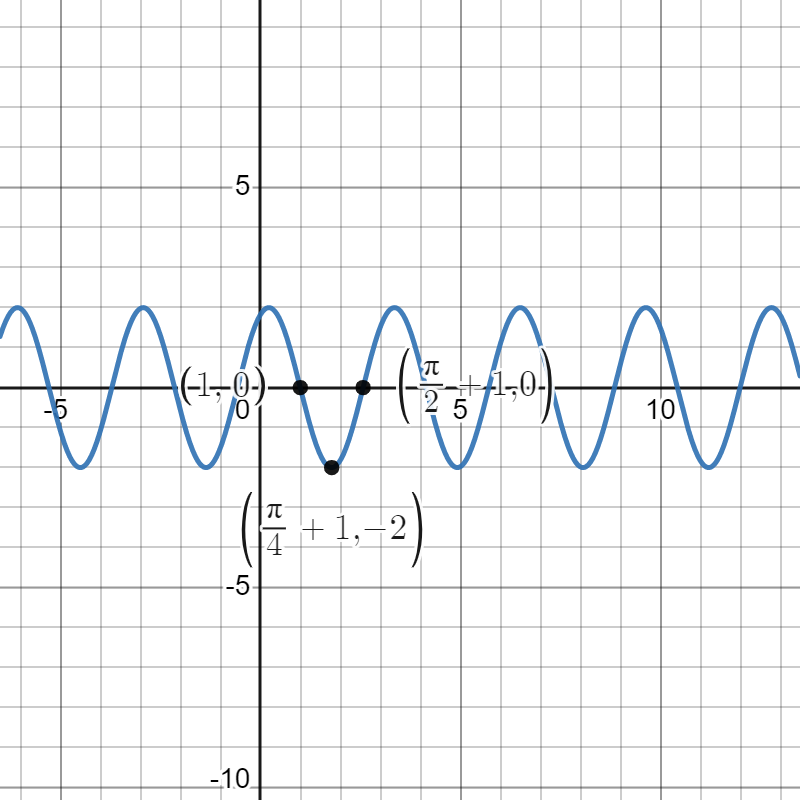
\includegraphics[width=0.8\linewidth]{images/graph-2-ex4.png}
\end{image}

Our final transformation is a shift up by 3 units, yielding $f_5(x) = f_4(x) + 3 = -2\sin(2x - 2) + 3$. This transforms our points into $(2, 3)$, $\left(\frac{\pi}{4} + 1, 1 \right)$, and $\left(\frac{\pi}{2} + 1, 3\right)$.  We can see a graph of $f_5$ below.
\begin{image}
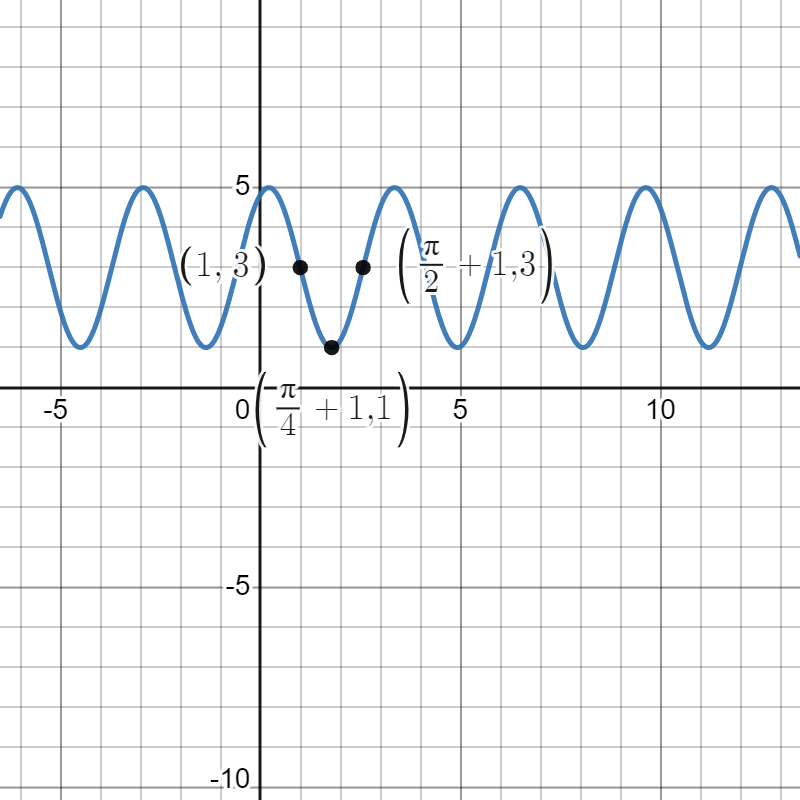
\includegraphics[width=0.8\linewidth]{images/graph-2-ex5.png}
\end{image}

The midline of $f$ is 3, the amplitude is 2, and the period is $\pi$. This is all readable from the graph, but also from the formula for $f$, since $|a| = 2$, $b = 2$, and $k = 3$. 
\end{explanation}
\end{example}

You may have noticed that the last example involved a reflection, a transformation we have not talked about in the context of circular functions. This is because reflections of circular functions turn out to be obtainable by shifts, so when we're given graphical information and asked to reconstruct the formula for a function, we don't need to use reflections. Reflections may show up when we are given a formula and asked to provide a graph. But we already have lots of practice producing graphs in this situation and can draw on this prior experience with transformations. 

%
%
%\typeout{************************************************}
%\typeout{Subsection 2.4.4 Summary}
%\typeout{************************************************}
%

\begin{summary}
\begin{itemize}[label=\textbullet]
\item
Given real numbers \(a\), \(h\), and \(k\) with \(a > 0\), the functions%
\begin{equation*}
f(t) = a\cos(t-h)+k \text{ and } g(t) = a\sin(t-h) + k
\end{equation*}
each represent a horizontal shift by \(h\) units to the right, followed by a vertical stretch by \(a\) units, followed by a vertical shift of \(k\) units, applied to the parent function (\(\cos(t)\) or \(\sin(t)\), respectively).  The resulting circular functions have midline \(y = k\), amplitude \(a\), range \([k-a,k+a]\), and period \(P = 2\pi\).  In addition, the anchor point \((h,a+k)\) lies on the graph of \(f\) and the anchor point \((h,k)\) lies on the graph of \(g\).%
\item
Given a function \(f\) and a constant \(b > 0\), the algebraic transformation \(h(t) = f(bt)\) results in horizontal scaling of \(f\) by a factor of \(b\).  In particular, when \(b > 1\), the graph of \(f\) is compressed toward the \(y\)-axis by a factor of \(b\) to create the graph of \(h\), while when \(0 < b < 1\), the graph of \(f\) is stretched away from the \(y\)-axis by a factor of \(b\) to create the graph of \(h\).%
\item
Given any circular periodic function for which the midline, amplitude, period, and an anchor point are known, we can find a corresponding formula for the function of the form%
\begin{equation*}
f(t) = a\cos(b(t-h))+k \text{ or } g(t) = a\sin(b(t-h)) + k\text{.}
\end{equation*}
Each of these functions has period midline \(y = k\), amplitude \(a\), and period \(P = \frac{2\pi}{b}\).  The point \((h,a+k)\) lies on \(f\) and the point \((h,k)\) lies on \(g\).%
\end{itemize}
\end{summary}
%
%

\end{document}